\begin{itemize}
    \item In der Regel ist zumindest ein kurzes Theoriekapitel notwendig. Es nimmt Bezug auf das thematische Oberthema, aber natürlich nicht auf allgemeine theoretische Grundlagen etwa aus der Naturwissenschaft.
\end{itemize}
The background chapter describes the theory of the approach and methods used in the thesis. In the first sections, the Formula SAE Competition, the \acrlong{ros}, and the autonomous system of \acrlong{zur} are introduced. After those sections, driverless as a concept will be introduced. In the end, several path planning algorithms are introduced and followed.

\section{Formula SAE Competitions} \label{sec:Formula SAE Competitions}
The main idea of a Formula SAE competition is to conceive, design, fabricate, develop and compete with small, formula-style race cars.
The competition is split into two classes: Internal Combustion Engine Vehicle (\acrshort{cv}) and Electric Vehicle (\acrshort{ev}).
Additionally, a team can opt-in to take part in the Driverless Cup (\acrshort{dc}).
After a series of technical inspections regarding safety and rules compliance, the vehicles will compete in a series of static and dynamic events. In the end, the team with the most overall points will win the competition for its class or the \acrlong{dc}, respectively. \cite{fs_rules_2022_handbook}
In a single Formula Student Germany competition, dozens of teams are participating, as shown in figure \ref{fig:FS SAE Competition}.
\begin{figure}[H]
    \centering
    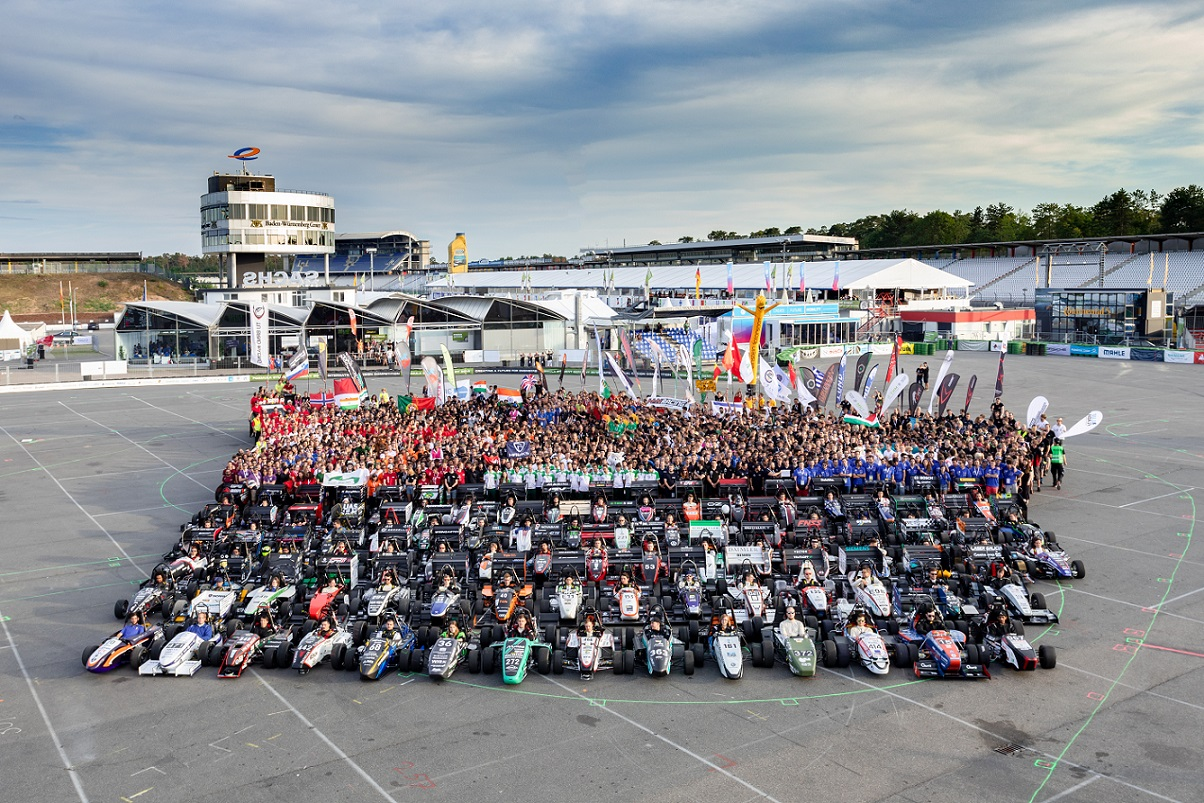
\includegraphics[width=\columnwidth]{FS_SAE_Competition.jpeg}
    \caption{Teams participating in Formula Student Germany. \cite{fs_germany}}
    \label{fig:FS SAE Competition}
\end{figure}

\subsection{Static Events} \label{sec:Static Events}
The following static events are held: Business Plan Presentation, Cost and Manufacturing, and Engineering Design. In these events, the engineers have to present their car and their development processes to a panel of judges. \cite{fs_rules_2022_handbook}

\textbf{Business Plan Presentation:} The team's ability to develop and deliver a comprehensive business model is evaluated. The presentation should demonstrate how their self-developed race car could become a profitable business idea.

\textbf{Cost and Manufacturing:} The financial planning of the car, including the manufacturing processes and costs associated with the construction of the race car, are evaluated.

\textbf{Engineering Design:} Evaluation of the engineering process and effort that went into the design of the vehicle. Technical aspects, the construction, and the car's key attributes are judged.

\subsection{Dynamic Events} \label{sec:Dynamic Events}
The following dynamic events are held: Skid Pad, Acceleration, Autocross, Endurance and Efficiency, and Track Drive.
The dynamic events reveal the driving performance of the prototypes. Every discipline puts different abilities of the cars to the test. \cite{fs_rules_2022_handbook}

\textbf{Skid Pad:} The skid pad track as shown in figure \ref{fig:FS Skid Pad layout} consists of two pairs of concentric circles in the shape of an eight. This track will test the lateral grip of the car.
\begin{figure}[H]
    \centering
    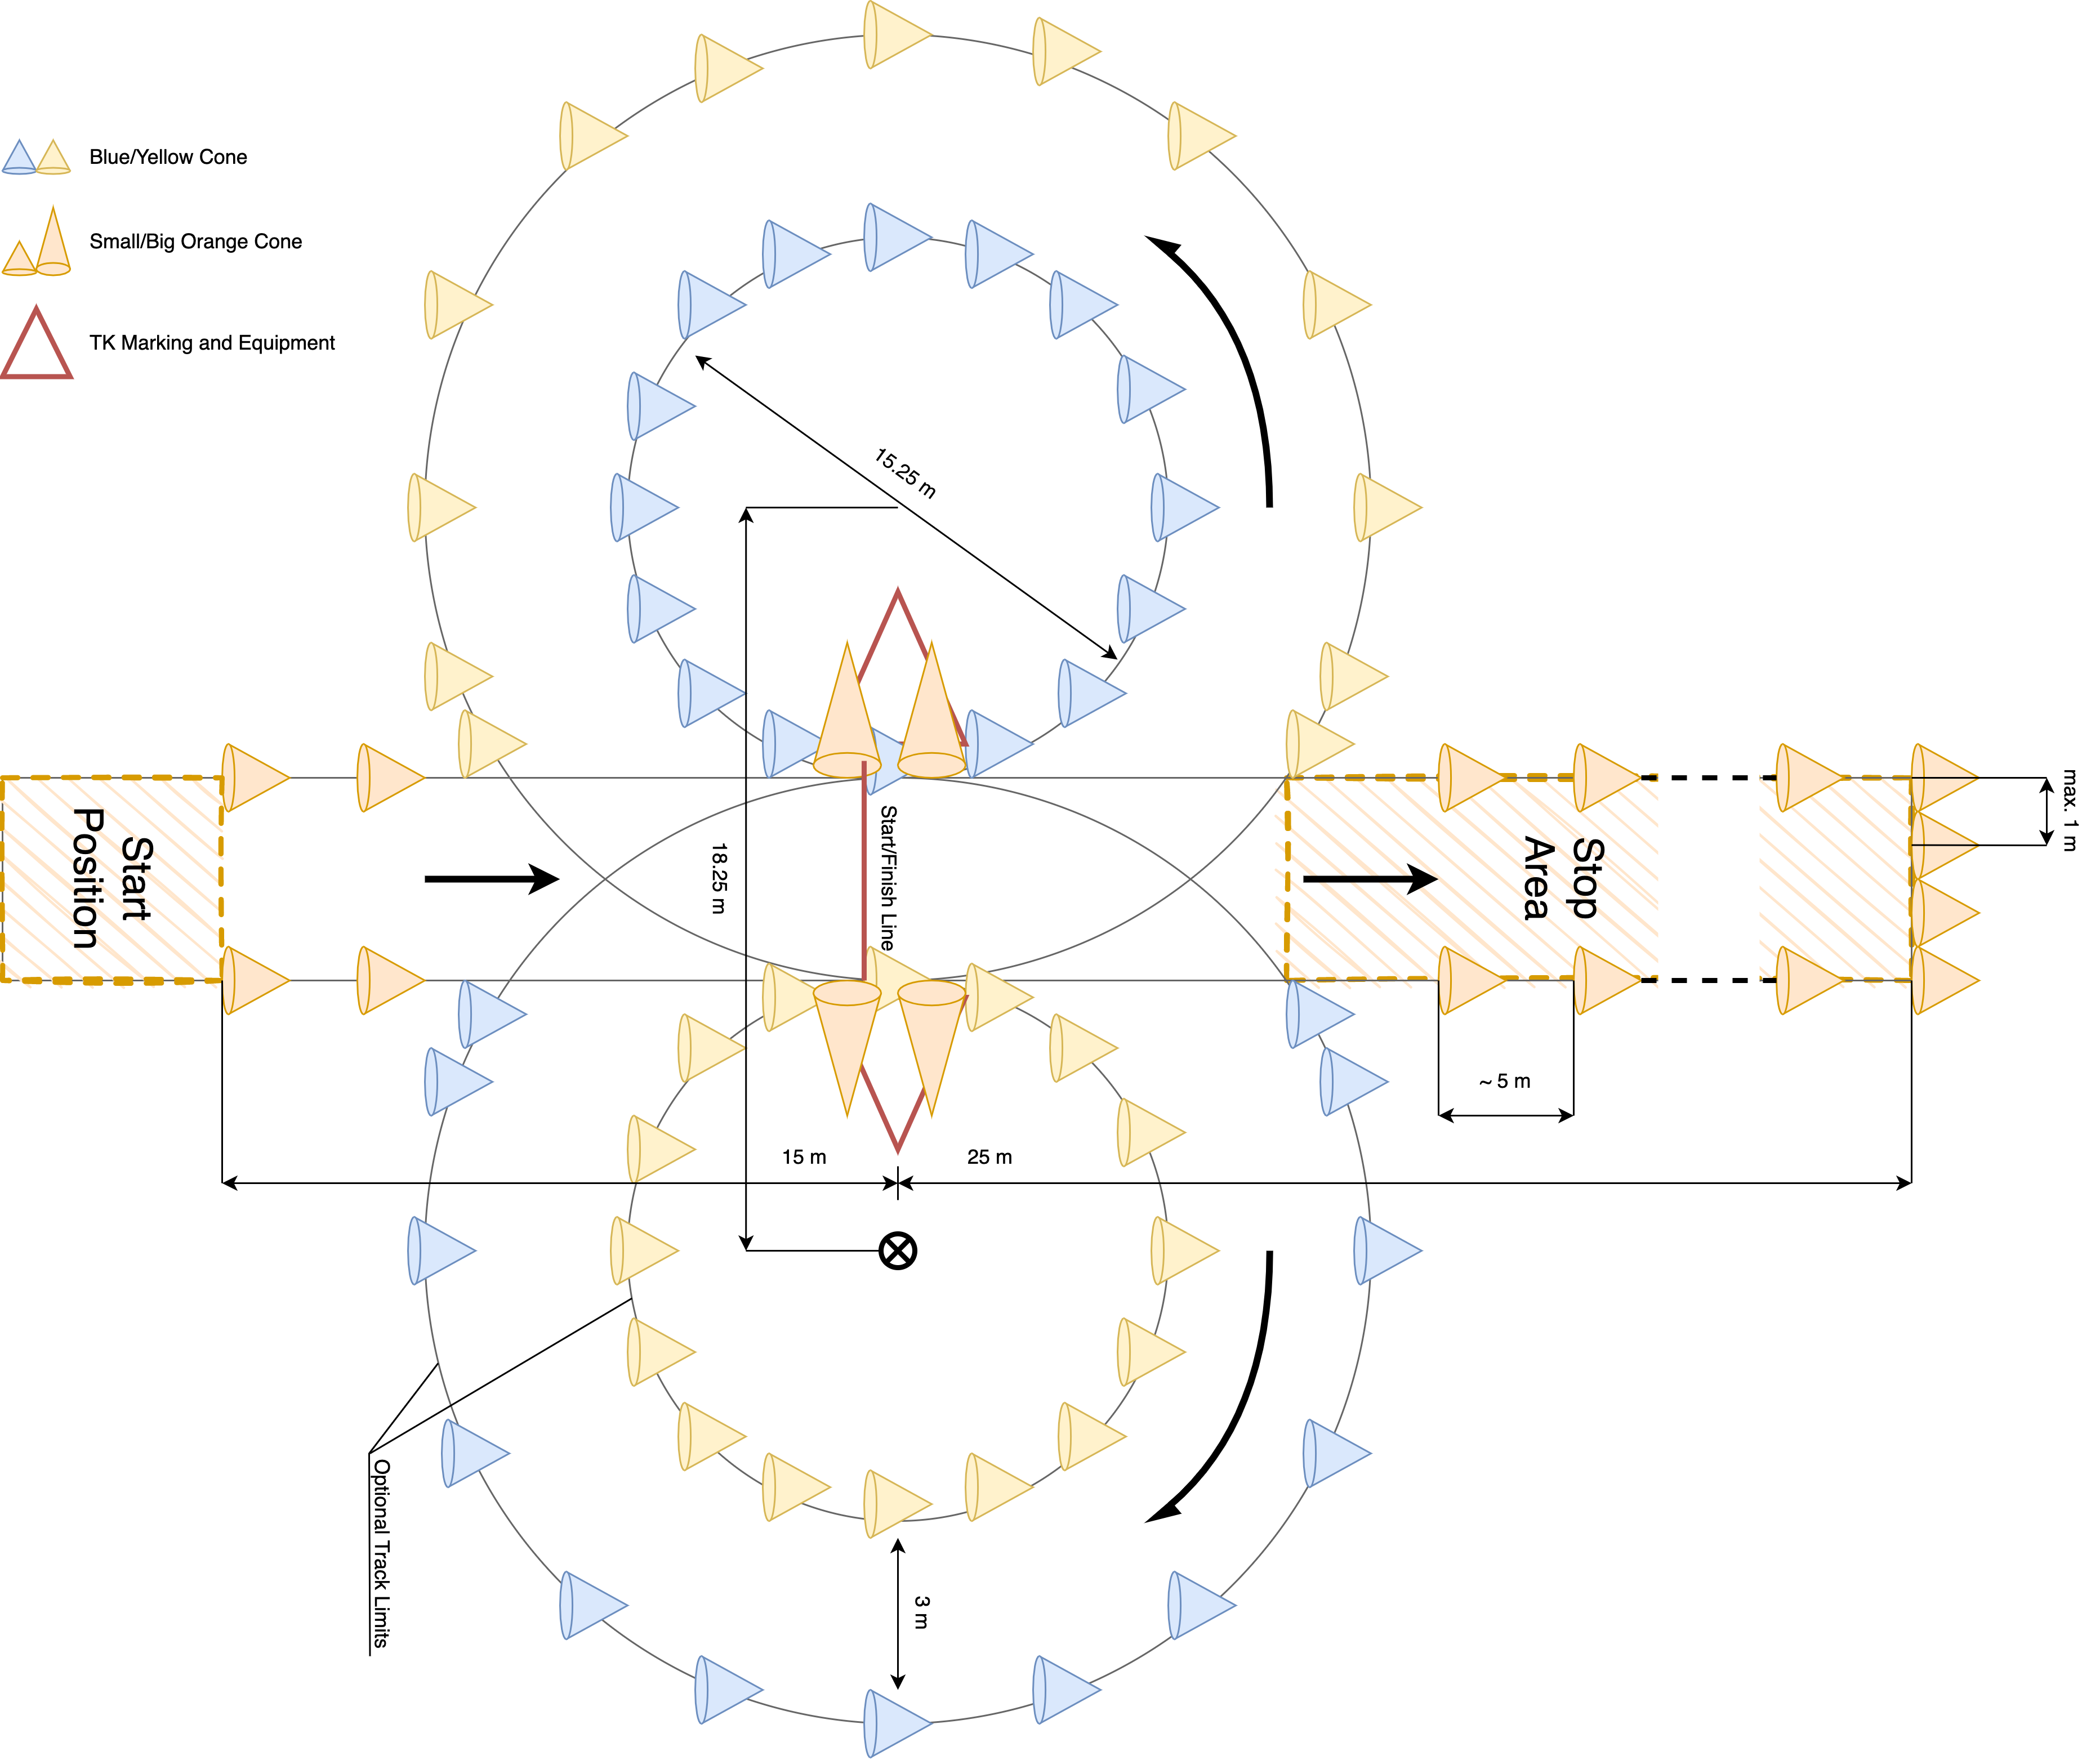
\includegraphics[width=\columnwidth]{FS_Event_Skid_Pad.png}
    \caption{Skid Pad track layout according to the Formula Student Rules 2022 handbook. \cite{fs_rules_2022_handbook}}
    \label{fig:FS Skid Pad layout}
\end{figure}

\textbf{Acceleration:} An acceleration race over 75 m distance as shown in figure \ref{fig:FS Acceleration layout} with a standing start, which tests the car acceleration in a straight line.
\begin{figure}[H]
    \centering
    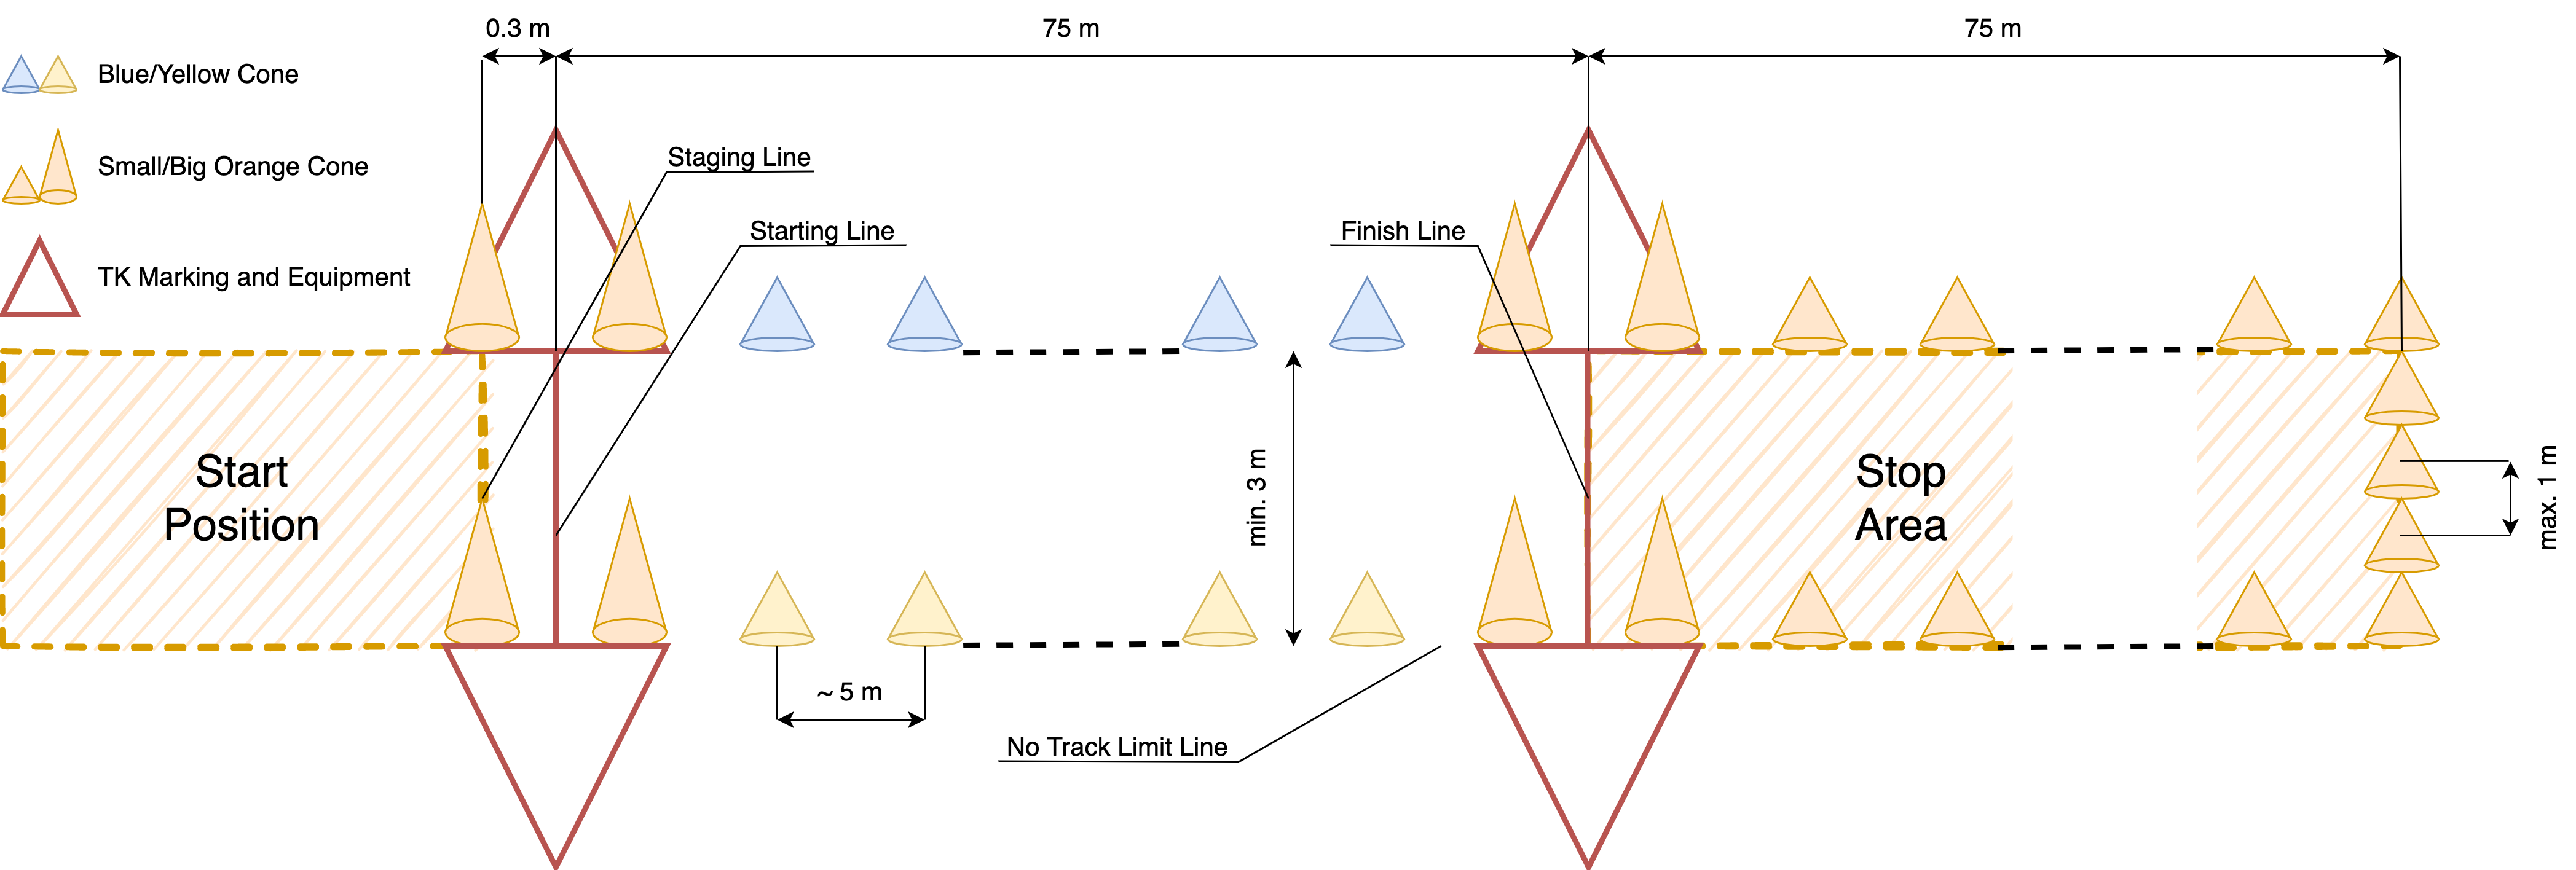
\includegraphics[width=\columnwidth]{FS_Event_Acceleration.png}
    \caption{Acceleration track layout according to the Formula Student Rules 2022 handbook. \cite{fs_rules_2022_handbook}.}
    \label{fig:FS Acceleration layout}
\end{figure}

\textbf{Autocross:} The autocross event tests the car's dynamic ability in a one-lap sprint. The objective of the autocross event is to evaluate the car's manoeuvrability and handling qualities.

\textbf{Endurance and Efficiency:} An endurance race over a distance of 22 km, including one driver change. One lap of the endurance track is approximately 1 km. The Efficiency scoring rates the consumed amount of energy to the total time.

\textbf{Trackdrive (DC Only):}  Over a distance of 10 rounds, the car has to prove its durability without a driver under long-term conditions. As shown in figure \ref{fig:FS Autocross, Endurance and Trackdrive layout} a basic layout is given as a reference.
\begin{figure}[H]
    \centering
    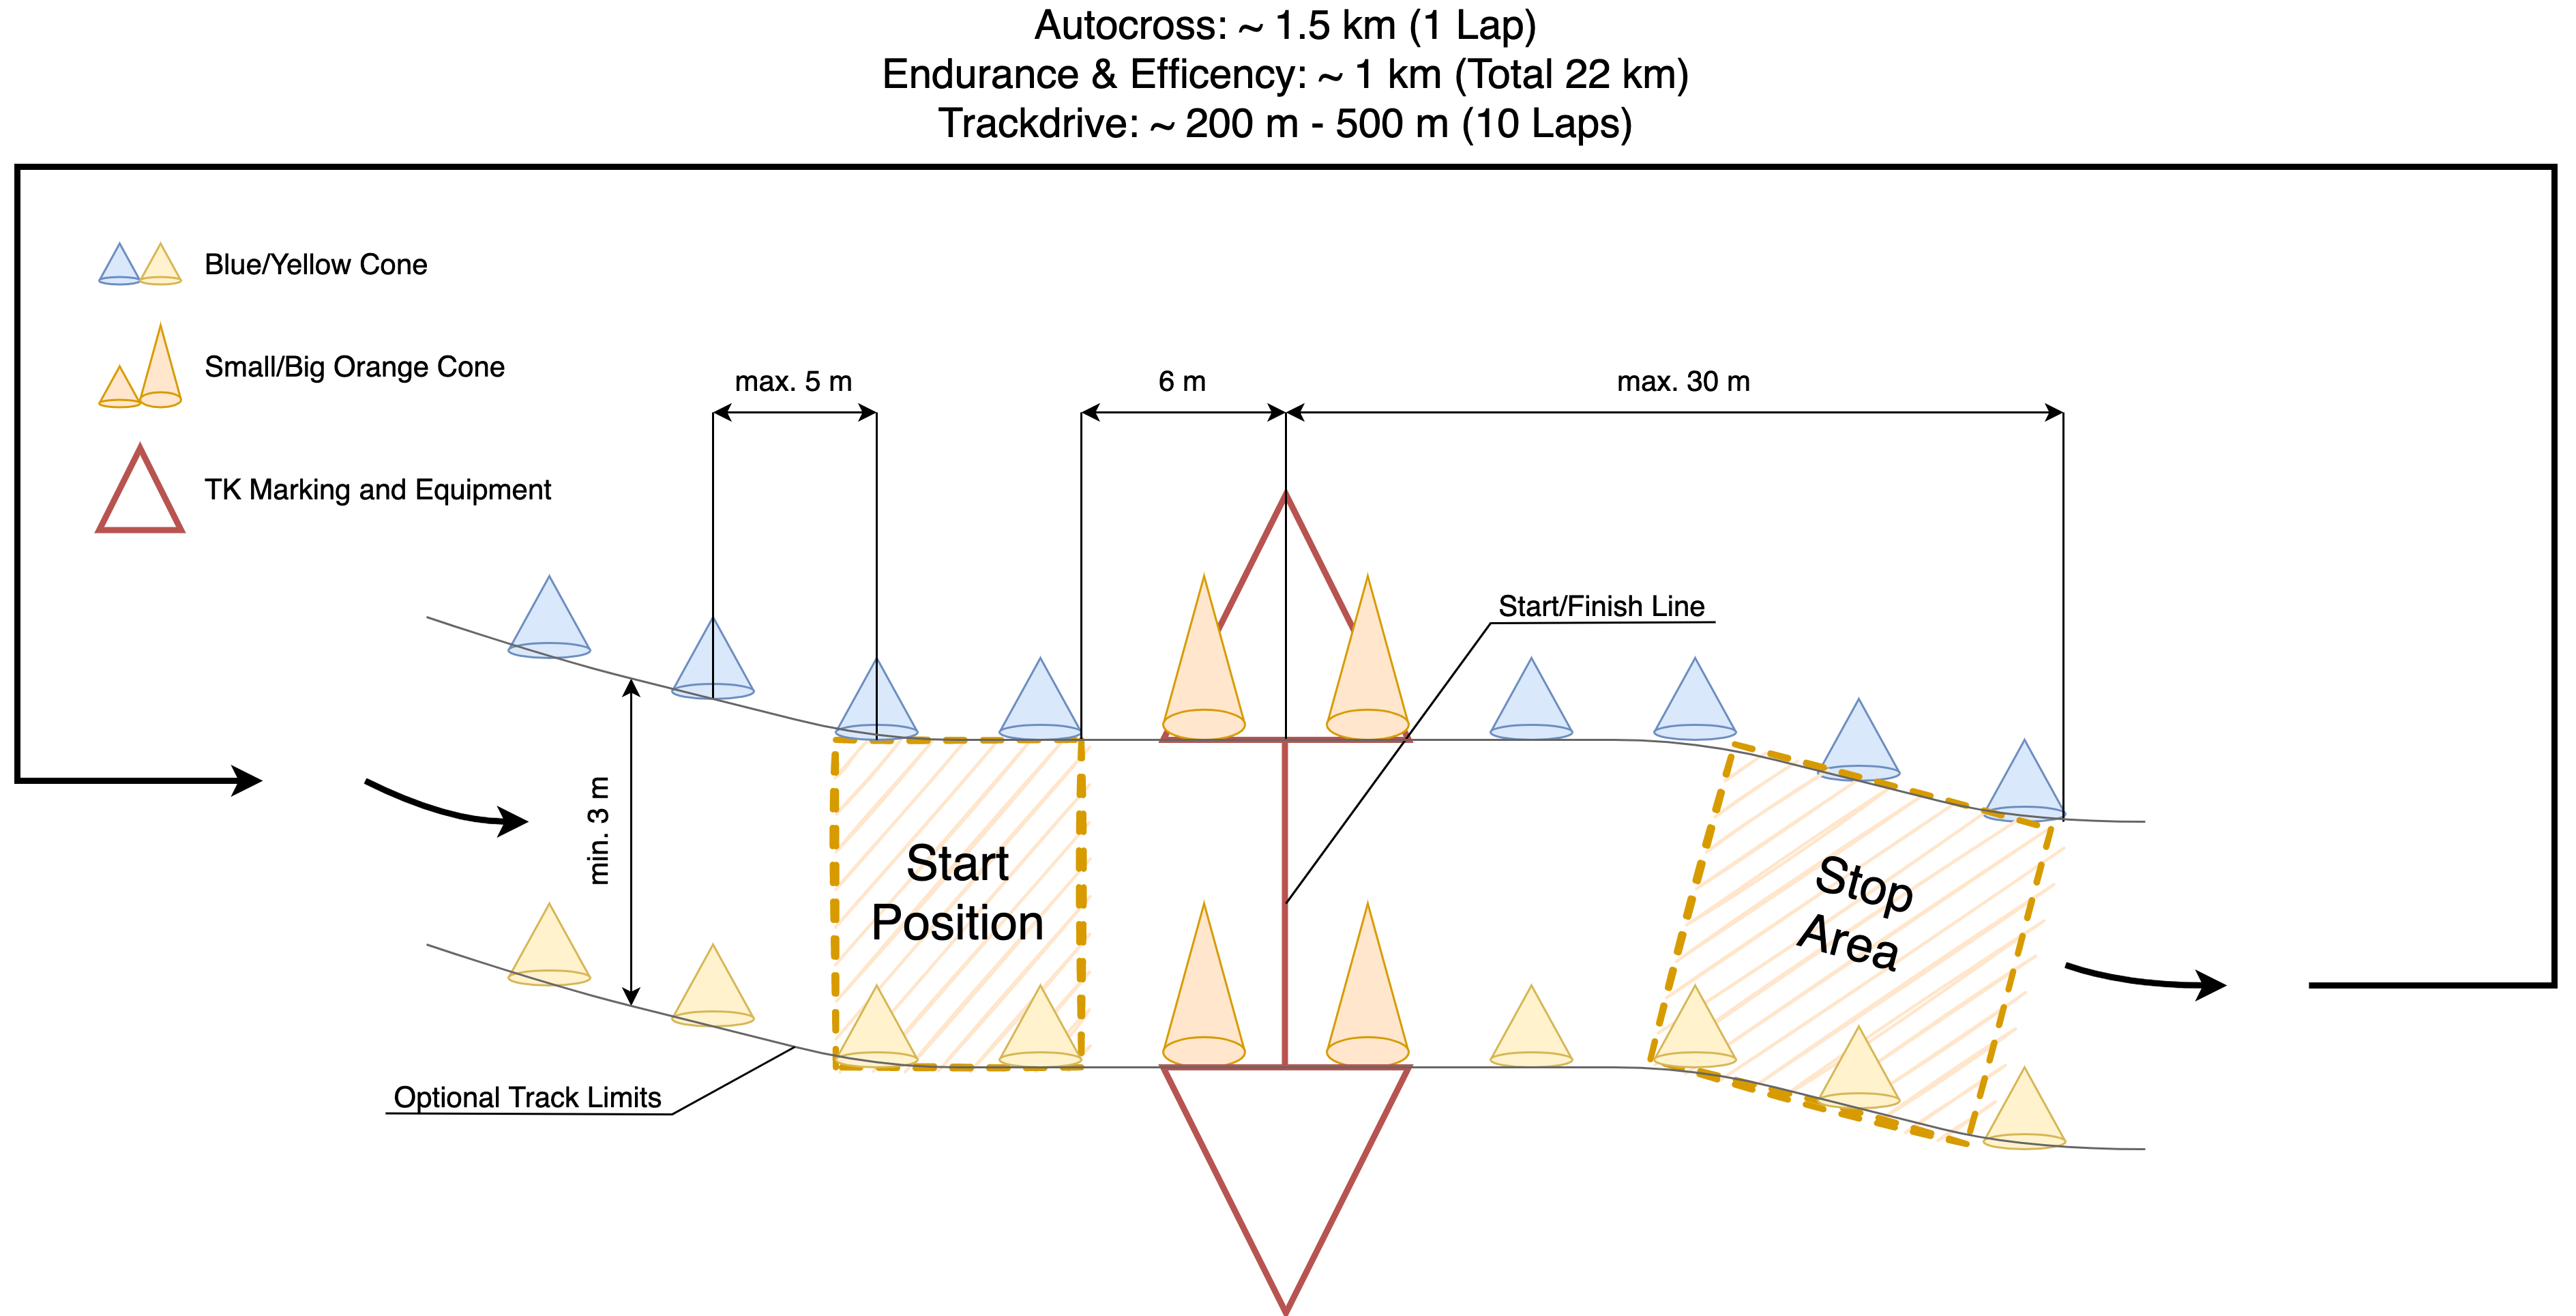
\includegraphics[width=\columnwidth]{FS_Event_Trackdrive.png}
    \caption{Base layout for the Autocross, Endurance and Trackdrive events according to the Formula Student Rules 2022 handbook. \cite{fs_rules_2022_handbook}}
    \label{fig:FS Autocross, Endurance and Trackdrive layout}
\end{figure}

\section{Robot Operating System (ROS)} \label{sec:Robot Operating System (ROS)}
The \acrlong{ros} (\acrshort{ros}) is not, like the name may suggest, a full-fledged operating system but a set of software libraries and tools for the development of robot applications. The open-source robotics middleware comes shipped with capable developer tools, drivers, and advanced algorithms. \cite{ros2_documentation}

There are currently two major versions of \acrshort{ros} which are seeing releases, ROS 1 and ROS 2. \cite{ros2_documentation} Beginning with releases after 'Foxy Fitzroy', releases in odd years will be non-LTS (Long Term Support). They will only be supported for 1.5 years, while new releases in even years will be supported long-term for five years. \cite{ros2_documentation}

\subsection{ROS Graph} \label{sec:ROS Graph}
Five main concepts of ROS 2 make up the ROS (2) graph:
\begin{enumerate}
    \item Nodes
    \item Topics
    \item Services
    \item Parameters
    \item Actions
\end{enumerate}

The ROS graph is a network of ROS 2 elements that process data simultaneously. The graph encompasses all executables and the connections between them.

\begin{figure}[H]
    \centering
    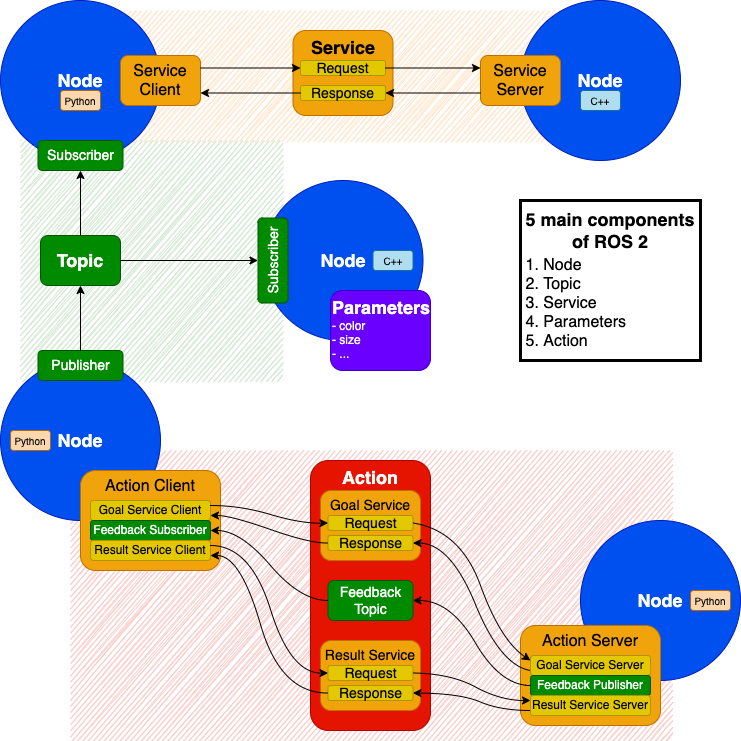
\includegraphics[width=\columnwidth]{ROS2_Main_Concepts.png}
    \caption{The five main concepts of ROS 2 pictured as a network of nodes.}
    \label{fig:ROS 2 main concepts}
\end{figure}

\subsubsection{Nodes} \label{sec:ROS Nodes}
A node is a fundamental ROS 2 element that serves a single modular purpose in a robotics system. \cite{ros2_documentation}

\subsubsection{Topics} \label{sec:ROS Topics}
Nodes publish information over topics, which allows any number of other nodes to subscribe to and access that information. \cite{ros2_documentation}

\subsubsection{Services} \label{sec:ROS Services}
Services are based on a call-and-response model versus topics’ publisher-subscriber model. Services only provide data when a client calls them explicitly. \cite{ros2_documentation}

\subsubsection{Parameters} \label{sec:ROS Parameters}
Nodes have parameters to define their default configuration values. \cite{ros2_documentation}

\subsubsection{Actions} \label{sec:ROS Actions}
Actions are built on topics and services and consist of a goal, feedback, and a result. Actions are like services that allow someone to execute long-running tasks, provide regular feedback, and are cancellable. \cite{ros2_documentation}

\section{Zurich UAS Racing Autonomous System} \label{sec:Zurich UAS Racing Autonomous System}
On a high-level view, the 'Autonomous System' is made up of five domains: the 'Controls', 'Perception', 'Localization and Mapping', 'Path planning' as well as 'Simulation'. Figure \ref{fig:AS Component Diagram} shows an abstraction of how the different components interact with each other. %TODO Bild mehr beschreiben
\begin{figure}[H]
    \centering
    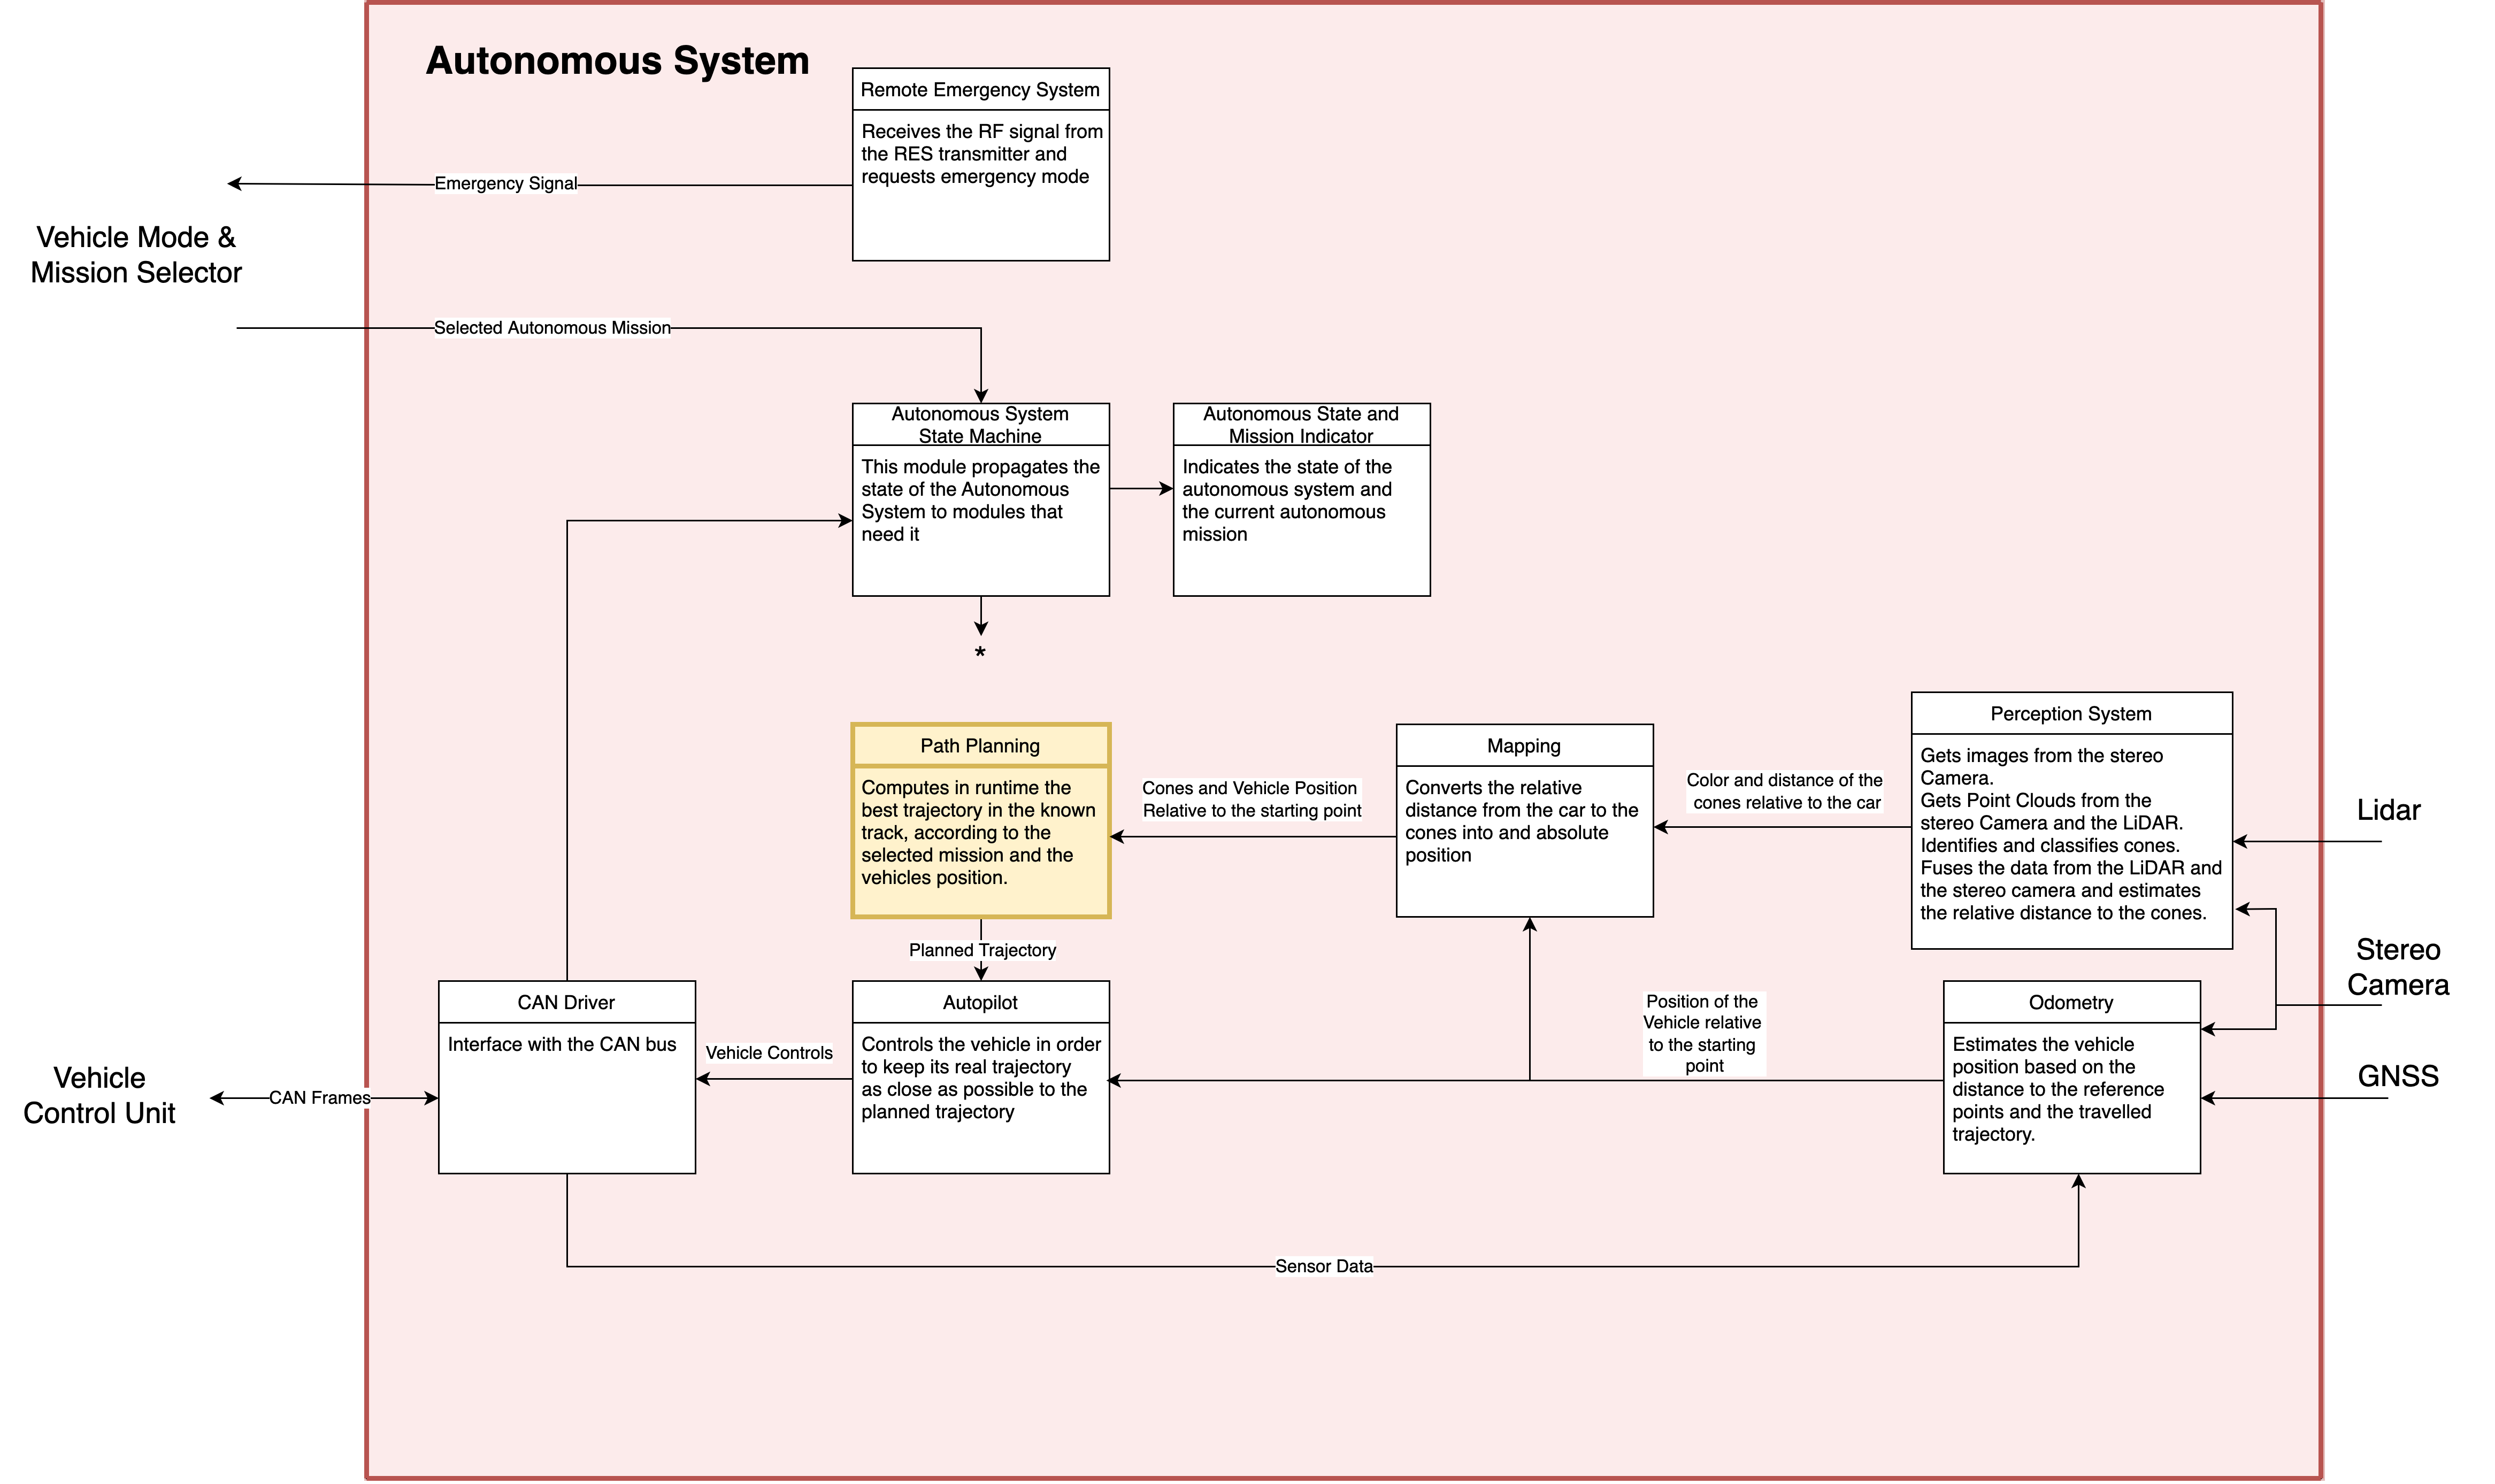
\includegraphics[width=\columnwidth]{AS_Component_Diagram.png}
    \caption{The Autonomous System Component Diagram shows an illustration between the hardware layer and software layer. The autonomous system (red box) is on the software layer, in which the 'Path Planning' domain (marked yellow) lies.}
    \label{fig:AS Component Diagram}
\end{figure}
The five domains are described as follows:
\textbf{'Controls'} is responsible for the steering, braking, and acceleration of the car.
\textbf{'Perception'} is recognizing the track by perceiving the different types of cones the track is made up of.
\textbf{'Localization and Mapping'} estimates the current position of the vehicle relative to the starting position and maps it into an absolute position on the track.
\textbf{'Path Planning'} computes the best possible path along the track.
\textbf{'Simulation'} is responsible for providing the rest of the domains with an adequate tool to simulate and test on.

Essential hardware components of the autonomous system are stored inside a box, which will be mounted on the vehicle itself. The connections coming into the box from the various components outside can be seen in the reference figure \ref{fig:AS DV Box}. %TODO Bild mehr beschreiben

\begin{figure}[H]
    \centering
    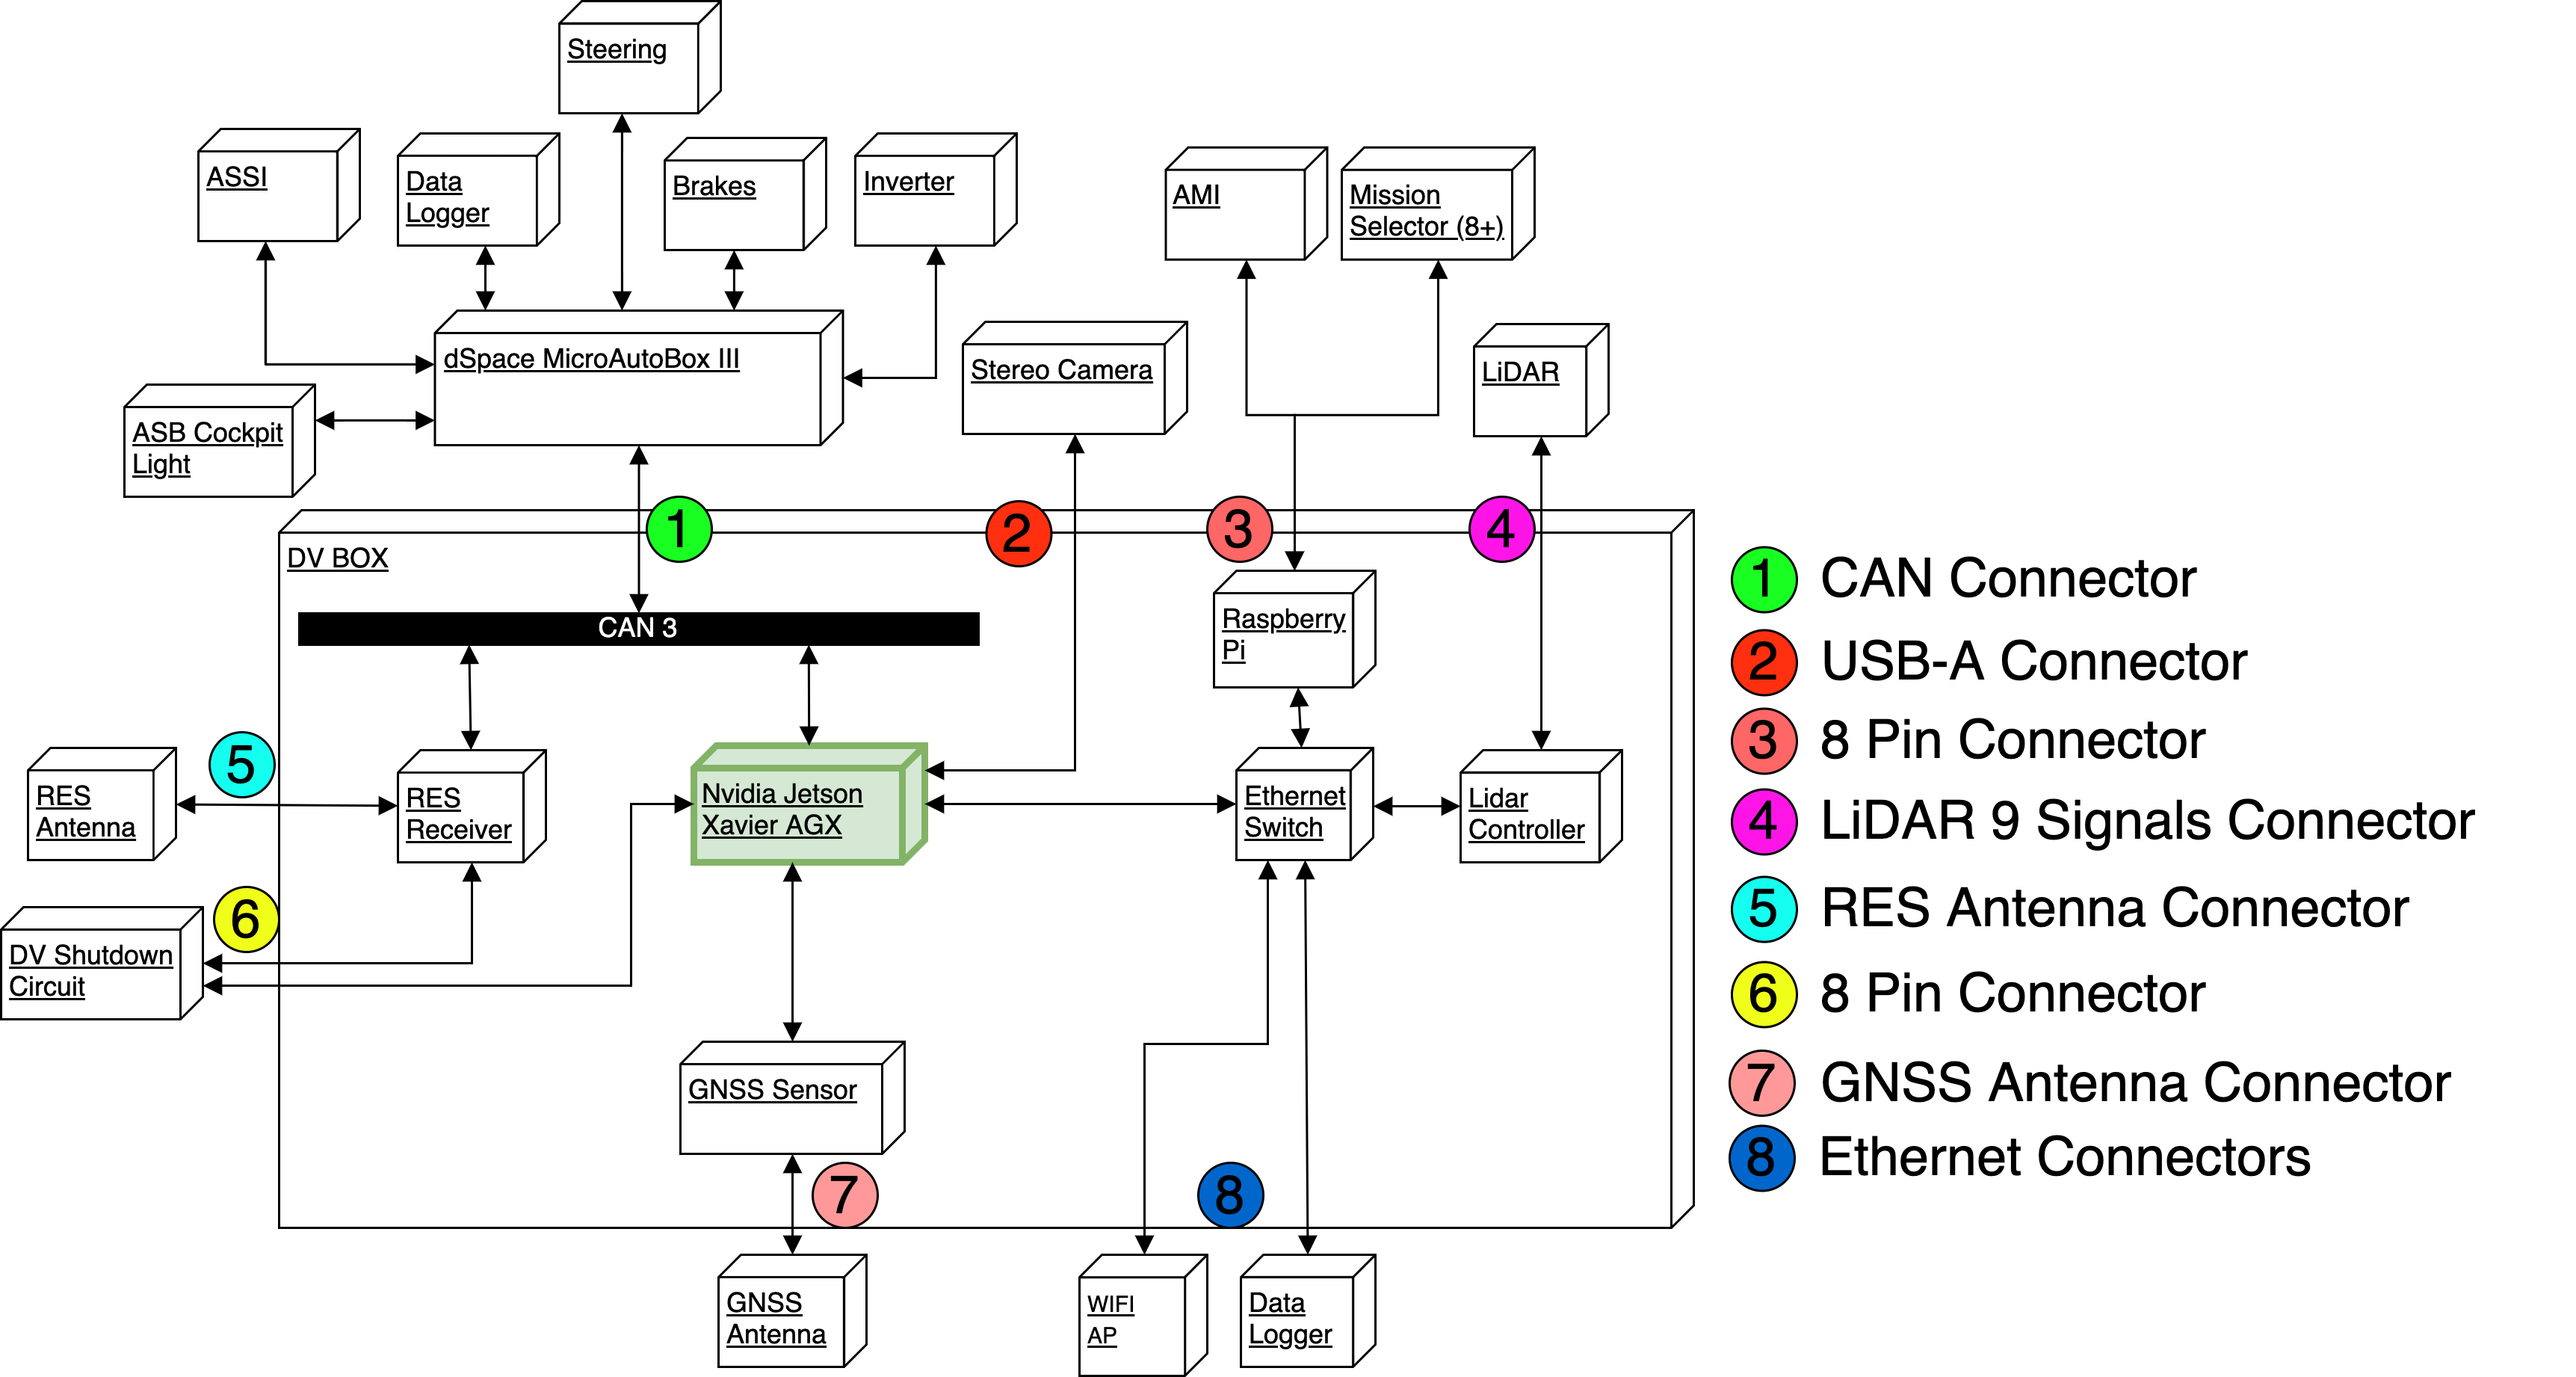
\includegraphics[width=\columnwidth]{AS_DV_Box.png}
    \caption{The Autonomous System DV Box consists of different components and connections to sensors, cameras and several other hardware components. The processing unit (marked in green) will house the software for the autonomous system itself.}
    \label{fig:AS DV Box}
\end{figure}

These components are shown in figure \ref{fig:AS HW Components}. Data needed for 'Localization' is received from the \acrshort{gnss} sensor and antenna (a MIKROE GNSS 7 Click and a u-blox ANN-MB). In contrast, the inputs for 'Perception' are received from the stereo camera (a Stereolabs ZED 2) and Lidar sensor (a Velodyne Lidar Puck Hi-Res), which are also needed for the 'Path Planning' module. Information for the 'Control' unit is sent over to the engine control unit (ECU) (a dSPACE MicroAutoBox III). In the end, all critical data for the operation leads into the processing unit of the system, which is, in this case, a 'Jetson AGX Xavier' by NVIDIA.
\begin{figure}[H]
    \centering
    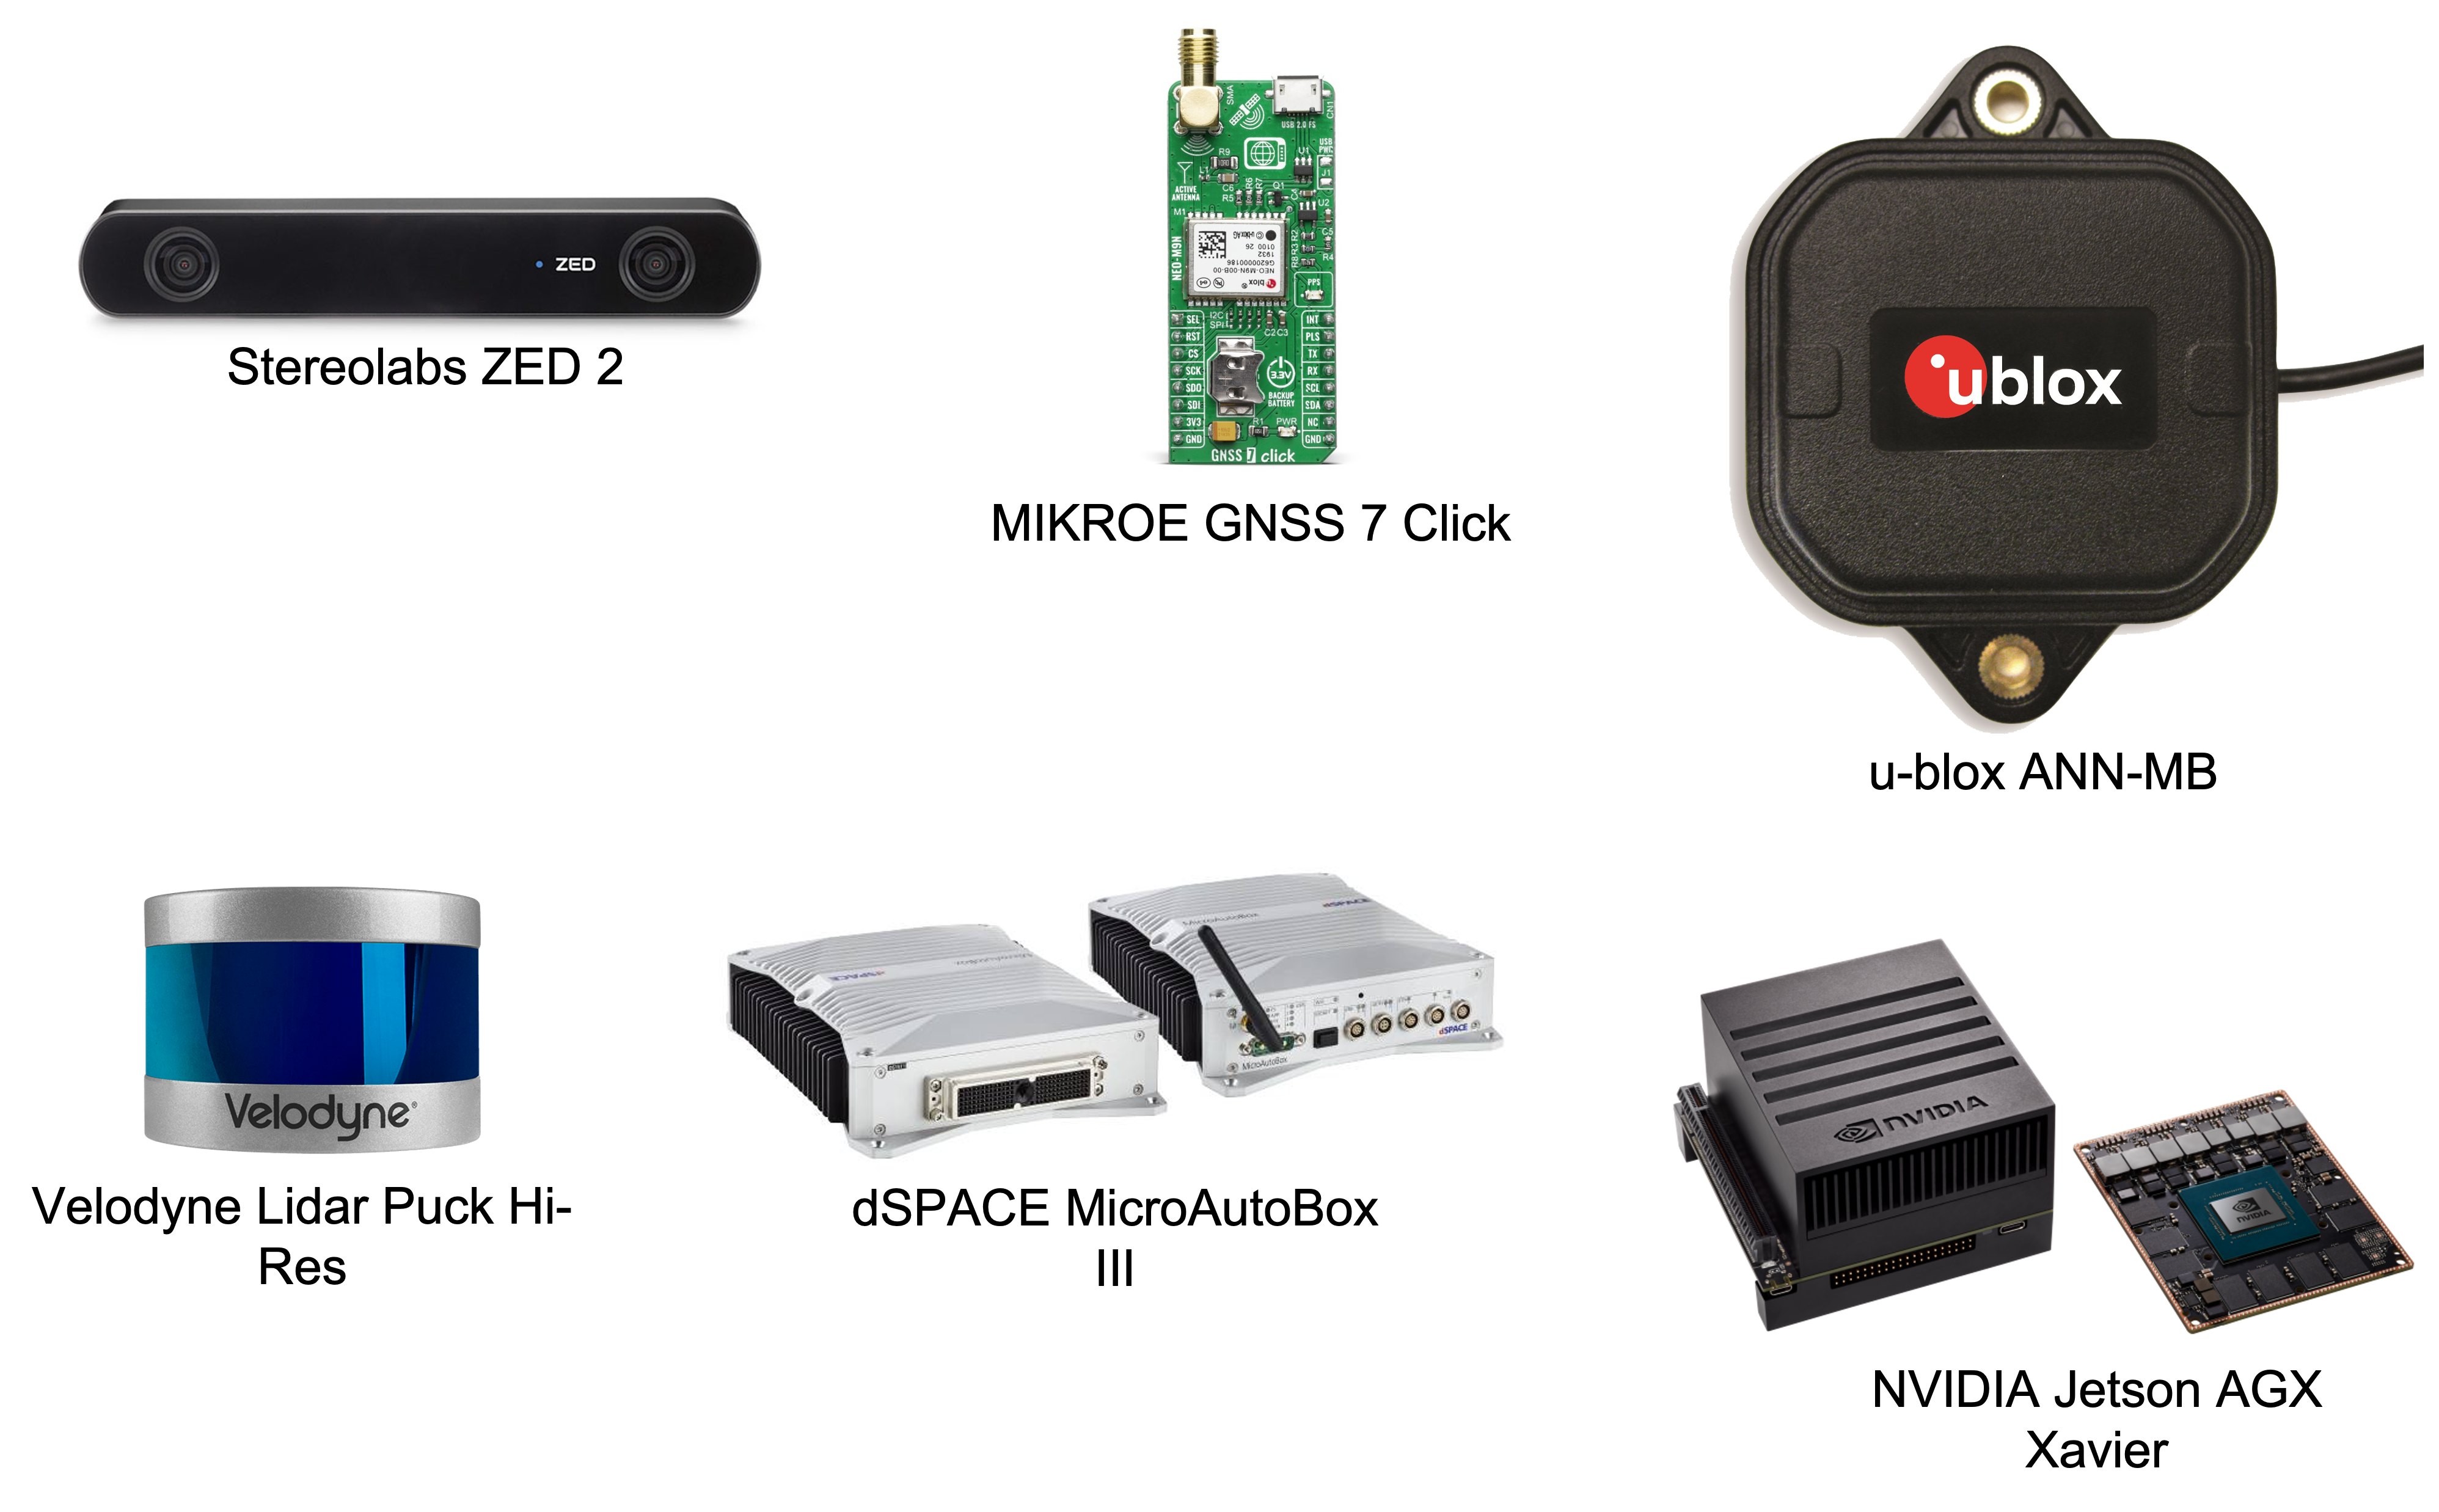
\includegraphics[width=\columnwidth]{AS_HW_Components.png}
    \caption{The Autonomous System Hardware Components consists of the Stereolabs ZED 2, MIKROE GNSS 7 Click, u-block AHN-MB, Velodyne Lidar Puck Hi-Res, dSPACE MicroAutoBox III and the NVIDIA Jetson AGX Xavier.}
    \label{fig:AS HW Components}
\end{figure}

The processing unit is set up with an installation of Ubuntu Linux 20.04, which will run the software of the autonomous system on top of \acrshort{ros}. Figure \ref{fig:AS Deployment Diagram} shows the levels of the software layers used.
\begin{figure}[H]
    \centering
    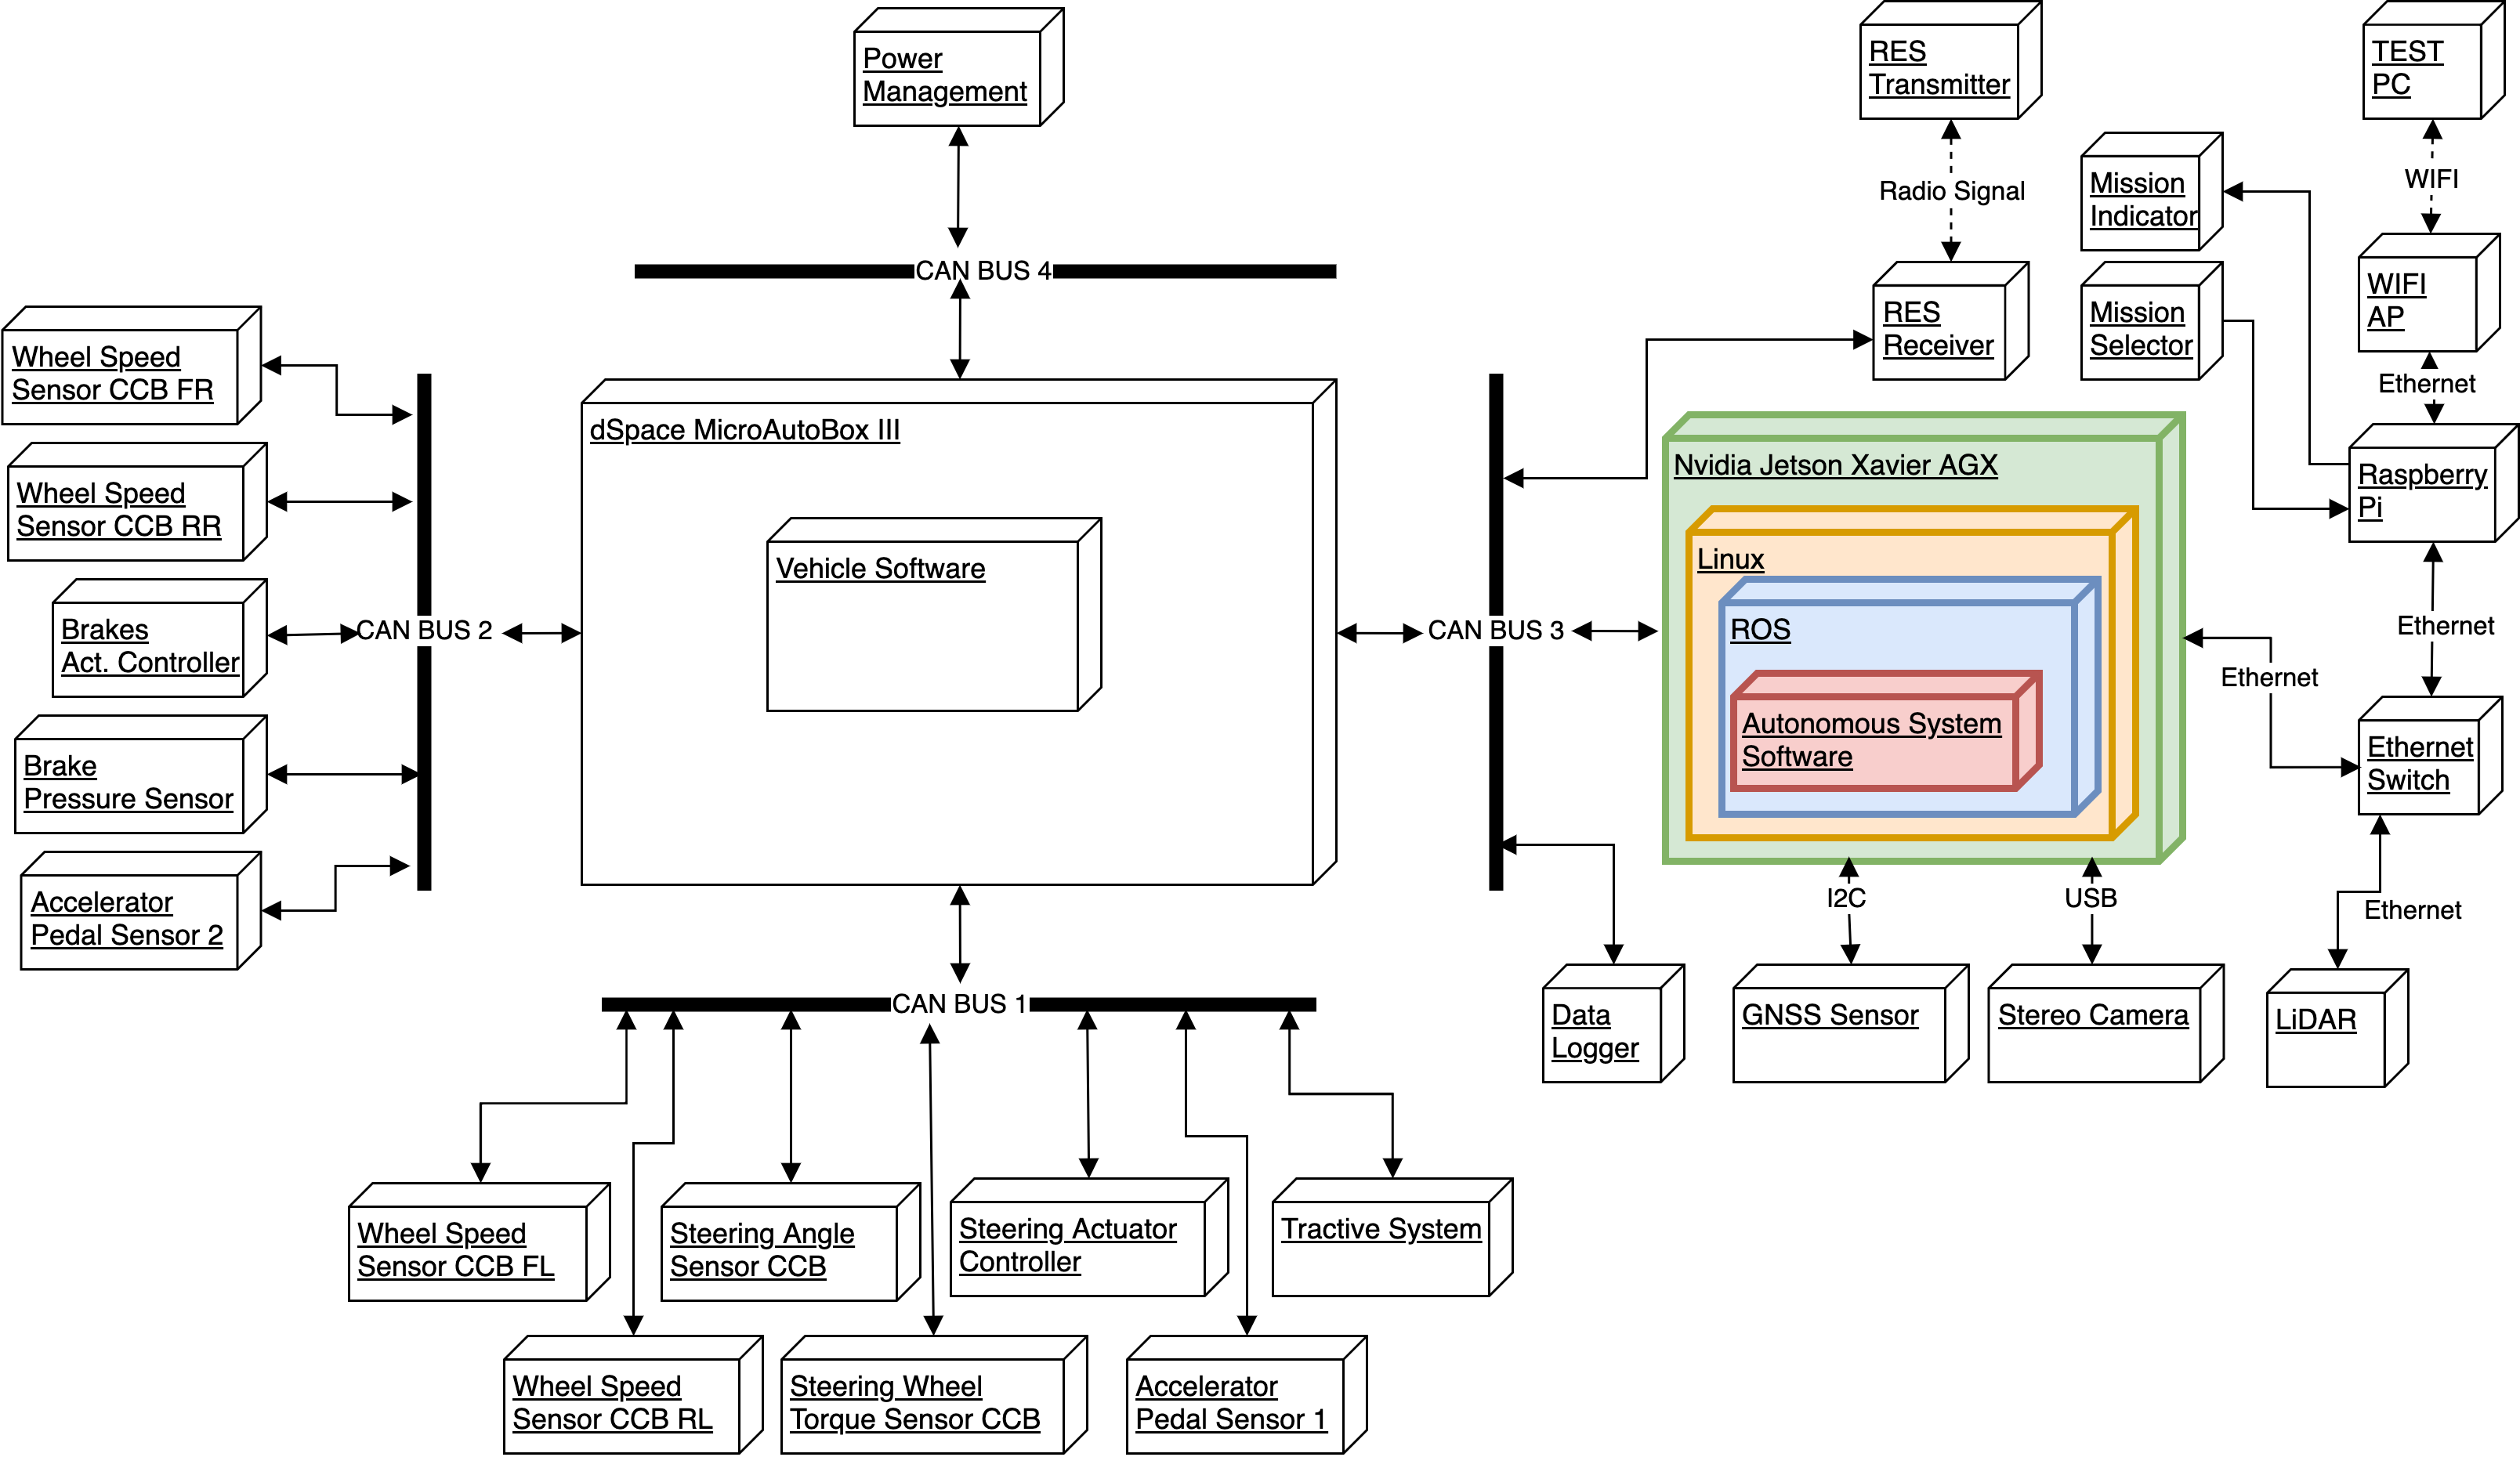
\includegraphics[width=6cm]{AS_Deployment_Diagram.png}
    \caption{The Autonomous System Deployment Diagram shows the different layers of software on the processing unit.}
    \label{fig:AS Deployment Diagram}
\end{figure}

\section{Driverless} \label{sec:Driverless}
The concept of driverless respectively an autonomous vehicle is a car incorporating vehicular automation, that is, a ground vehicle that is capable of sensing its environment and moving safely with little or no human input. \cite{driverless_cooperative_control}
Autonomous cars combine a variety of sensors to perceive their surroundings, such as cameras, radar, lidar, GPS, odometry and more. Control systems interpret sensory information to identify appropriate paths and obstacles and relevant signalizations. \cite{driverless_governing_autonomous_vehicles}

The \acrshort{sae} currently defines six levels of driving automation ranging from Level 0 (fully manual) to Level 5 (fully autonomous). \cite{driverless_sae_levels}
\begin{figure}[H]
    \centering
    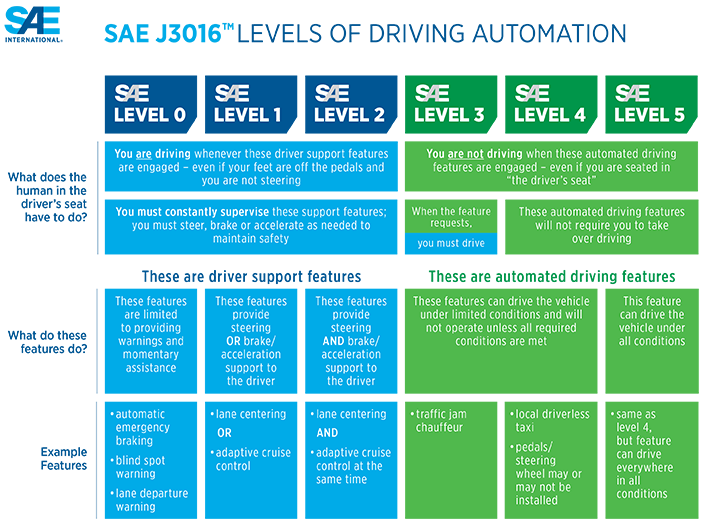
\includegraphics[width=\columnwidth]{Driverless_SAE_Levels.png}
    \caption{SAE J3016 defines the different levels of driving automation.}
    \label{fig:Driverless SAE Levels}
\end{figure}

Even with limitless scenarios for convenience and quality-of-life improvements and its potential for dramatically lowering CO2 emissions. \cite{driverless_study_three_revolutions}
Fully autonomous cars are still years away, as the challenges range from technological and legislative to environmental and philosophical. For example, lidar and radar scanners are still expensive and commonly used in current driverless cars. There is also the possibility of lidar signals interfering with each other or if the used radio frequency range will be enough to support the mass production of driverless cars. Additionally, there can be trouble with different traffic conditions. For example, how will the vehicle behave in tunnels or bridges? There are also additional hurdles like laws, regulations, and accident liability. \cite{driverless_what_is_an_autonomous_car}

Currently, we are largely still at level two according to \acrshort{sae}'s levels of driving automation, with cars able to control steering, acceleration and braking while still requiring drivers to remain engaged. Vehicles operating at Level 3 and above remain a marginal portion of the market. \cite{driverless_whats_the_status_of_self_driving_cars}
In March 2021, Honda became the first manufacturer to provide a legally approved Level 3 car and Toyota operated a potentially Level 4 service around the Tokyo 2020 Olympic Village. \cite{driverless_honda_sensing_elite} \cite{driverless_toyota_olympics}
\begin{figure}[H]
    \centering
    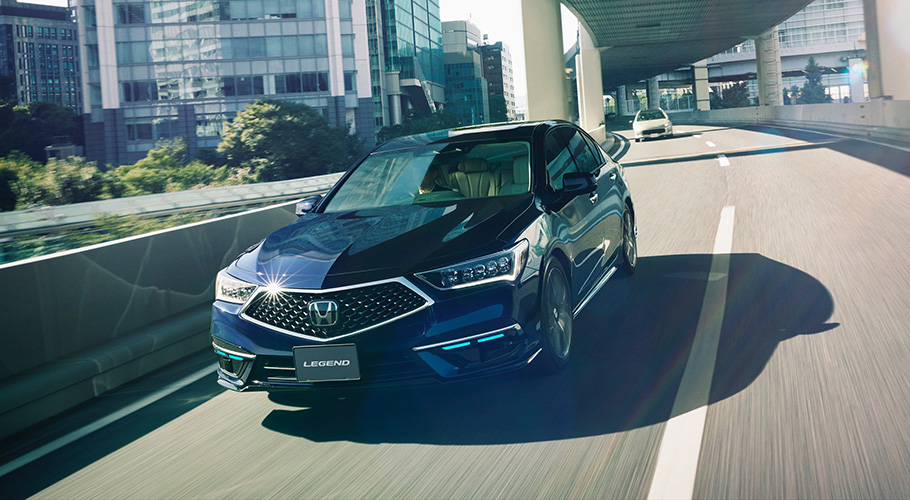
\includegraphics[width=12cm]{Driverless_Honda_Sensing_Elite.jpeg}
    \caption{The Honda Sensing Elite is the first legally approved Level 3 car according to the SAE's levels of driving automation in figure \ref{fig:Driverless SAE Levels}.}
    \label{fig:Driverless Honda Sensing Elite}
\end{figure}

\section{Path Planning Algorithms} \label{sec:Path Planning Algorithms}
Path planning algorithms are used in many environments, e.g. in the assembly of a car with a robot arm, in the autonomous parking of a car, or in finding a landmine with a robot during a military operation.

\subsection{Overview} \label{sec:Overview Path Planning Algorithms}
A human follows a path if it goes from point A to point B while following certain signalizations, e.g. on hiking trails. It also follows a path if it follows one predetermined for them by a GPS. The difference lies between a manual plan and a machine-generated plan. This section addresses the latter one.

The planning of a path consists of a state, the time needed, actions, an initial / goal state, a criterion, and a plan. A planning algorithm represents the state typically. Time is based on a sequence of decisions that must be made at a particular time. Actions manipulate the state and cover how the state should be changed. The initial and goal state defines where the planner should start and finish.
The criterion defines the outcome and the boundaries of the planner. The type of criterion is either based on feasibility or optimality. Feasibility covers the arrival of the goal state without the concern for efficiency. Optimality finds a plan with optimized performance in mind. The plan, in general, covers the strategy or behaviour of a decision-maker. \cite{planning_algorithms_steven_m_lavalle}

A path planning algorithm can be categorized into one of the following groups: Motion Planning, Decision-Theoretic Planning, and Planning under Differential Constraints.
\cite{planning_algorithms_steven_m_lavalle}

\subsection{Algorithms, Planners and Plans} \label{sec:Algorithms, Planners and Plans}
An algorithm usually consists of a machine and environment where there are actuations from the machine to the environment and sensing from the environment to the machine as shown in figure \ref{fig:Machine and Environment interaction}.
\begin{figure}[H]
    \centering
    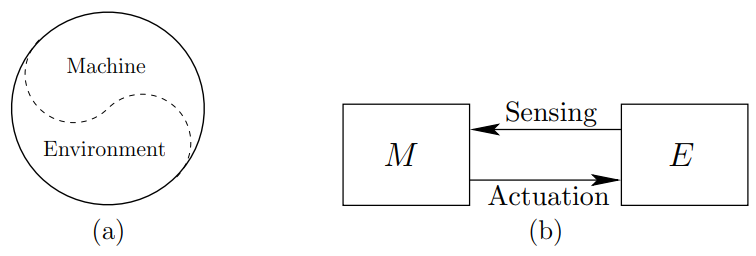
\includegraphics[width=10cm]{Machine_Environment.png}
    \caption{Two different illustrations that show what is the relationship between the machine and the environment. \cite{planning_algorithms_steven_m_lavalle}}
    \label{fig:Machine and Environment interaction}
\end{figure}
The problem in planning is often that the machine interacts with the physical world, which has uncountable different influences on the plan to be calculated. Because of this interaction with the physical world, the environment is often an approximation of the natural world since not every sensing mechanism can be processed from the environment to the machine.

Planners construct plans and are either a machine or a human. Should the planner be a machine, then a planning algorithm would be the planner. Should the planner be a human, the human itself would be the algorithm making the decisions. Figure \ref{fig:Planner Machine Environment} shows the interaction of a planner on a machine or a plan.
\begin{figure}[H]
    \centering
    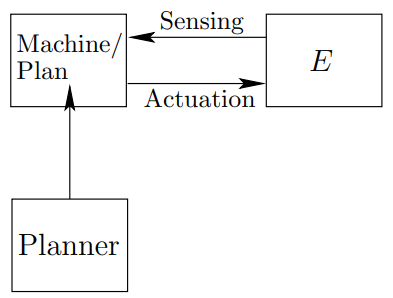
\includegraphics[width=5cm]{Planner_Machine_Environment.png}
    \caption{A planner executes the plan on the machine that actuates on the environment. \cite{planning_algorithms_steven_m_lavalle}}
    \label{fig:Planner Machine Environment}
\end{figure}

These plans can be used in three ways: Execution, refinement, or hierarchical inclusion. Execution runs the plan on a simulation or a robot connected to the real world. Refinement tries to find a better plan. Hierarchical inclusion hands over the plan to a higher level plan consisting of additional sub plans. \cite{planning_algorithms_steven_m_lavalle}

\subsection{Motion Planning} \label{sec:Motion Planning}
Motion planning is interested in the planning in continuous state spaces. This means that space is not static and will have changes with time. Motion planning is also referred to as planning in continuous state spaces. \cite{planning_algorithms_steven_m_lavalle}

\textbf{Implicit Representation} of state space in motion planning must be dealt with in planning algorithms. Implicit representations become more important in motion planning as the state space is uncountably infinite. It also tries to define 2D and 3D geometric models and transform them. The state spaces arise from these problems. \cite{planning_algorithms_steven_m_lavalle}
%TODO werden die verwendeten Begriffe wieder erwähnt?

\textbf{Continuous $\rightarrow$ discrete} is the central theme in motion planning to transform models. Motion planning also covers combinatorial motion planning, where the algorithm builds a representation of the original problem with an input model. Additionally, there exists also the field of sampling-based motion planning. \cite{planning_algorithms_steven_m_lavalle}

\textbf{Geometric Representation and Transformation} to start defining a motion planning algorithm. It defines a system's body in a space and how it transforms, e.g. moves. Movements can be chained in a state. \cite{planning_algorithms_steven_m_lavalle}

\textbf{The Configuration Space} is needed for the motion planning algorithm to define the space in which a set of possible transformations could be applied to the robot. \cite{planning_algorithms_steven_m_lavalle}

\textbf{Sampling-Based Motion Planning} is a field in motion planning that covers sampling-based algorithms. Sampling-based planning algorithms use collision detection as a "black box" separated from the geometric and kinematic models of motion planning. There are two different types of algorithm models. First, the single-query algorithm consists of a ($q_i,q_G$) pair as an input. $q_i$ defines the start and $q_G$ the end goal. In this strategy, no pre-computation is possible. Figure \ref{fig:Geometric Models Collision Detection Algorithm} illustrates the interaction between the geometric models, collision detection, the sampling-based motion planning algorithm, and the discrete searching method.
\begin{figure}[H]
    \centering
    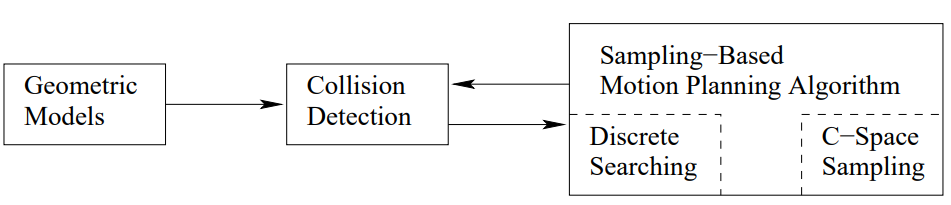
\includegraphics[width=\columnwidth]{Sampling-Based_Motion_Planning.png}
    \caption{The geometric models will generate the input for the collision detection, that influences the discrete searching in the sampling-based motion planning algorithm. The C-space is the configuration space of the algorithm. \cite{planning_algorithms_steven_m_lavalle}}
    \label{fig:Geometric Models Collision Detection Algorithm}
\end{figure}
A multi-query algorithm can have multiple initial goals; that is when it makes sense to precompute the models for more efficiency. An example of a single-query algorithm is the \acrshort{rdt} algorithm , similar to the \acrshort{rrt} algorithm mentioned in \ref{sec:Related Work}, which is a subset of the \acrlong{rdt} (\acrshort{rdt}) algorithm. It searches for the shortest path by creating random sequences that end up in a tree, which holds multiple sequences that can be connected. Figure \ref{fig:Rapidly Exploring Dense Tree} illustrates a simple example how a \acrshort{rdt} works.
\begin{figure}[H]
    \centering
    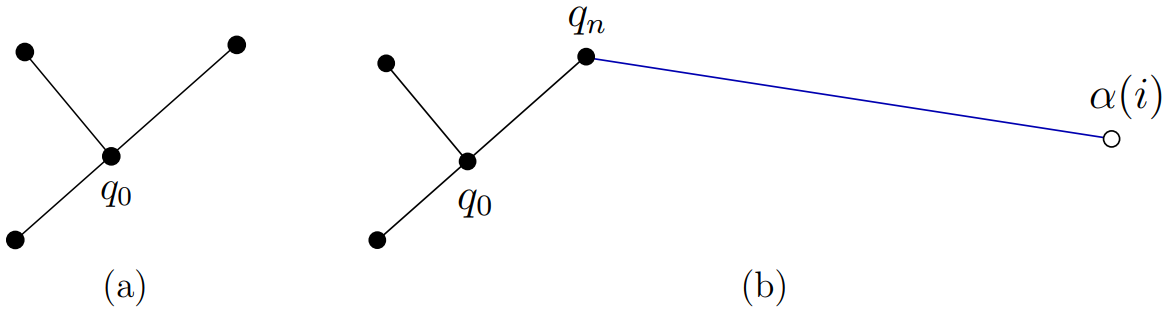
\includegraphics[width=\columnwidth]{Rapidly_Exploring_Dense_Tree.png}
    \caption{$q_0$ is the initial position and $q_n$ the vertex. $\alpha(i)$ is the sample based on the nearest point in $S$. (a) shows the tree that has been constructed and (b) the tree after applying the algorithm. \cite{planning_algorithms_steven_m_lavalle}}
    \label{fig:Rapidly Exploring Dense Tree}
\end{figure}

Listing \ref{lst:Simple RDT} shows a pseudocode implementation of the \acrshort{rdt} algorithm.
\begin{lstlisting}[mathescape=true, caption={The simple \acrshort{rdt} computes a random tree with the nearest function. \cite{planning_algorithms_steven_m_lavalle}}, label={lst:Simple RDT}]
SIMPLE RDT($q_0$)
 1 G.init($q_0$);
 2 for i = 1 to k do
 3 G.add vertex($\alpha(i)$);
 4 $q_n \rightarrow$ nearest(S(G), $\alpha(i)$);
 5 G.add edge($q_n$, $\alpha(i)$);
\end{lstlisting}
The goal of the multi-query method is the creation of a roadmap for each $q_i$ and $q_G$ and is the reason why the family of the algorithm is called a sampling-based roadmap. \cite{planning_algorithms_steven_m_lavalle}

\textbf{Combinatorial Motion Planning} covers the discovery of a path in a continuous space without resorting to approximations. Cell decompositions and cylindrical algebraic decomposition are two different subcategories of combinatorial motion planning algorithms. Cell decompositions are based on a collection of cells called a complex. In the 2D decomposition field exists a triangulation algorithm performed by vertical decomposition. The algorithm connects every built triangle with three nodes at a time. With four nodes, two triangles are made. Figure \ref{fig:Theory of Triangulation} gives an example of how the edges from the result of the triangulation are connected through the middle points.
\begin{figure}[H]
    \centering
    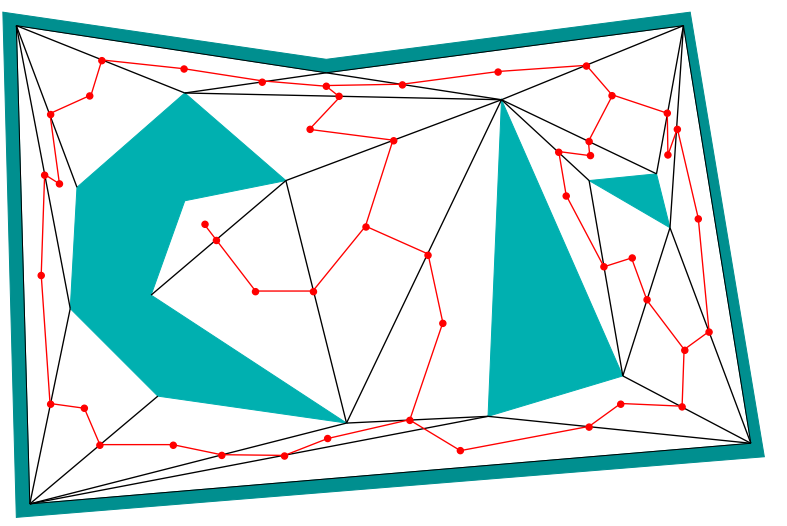
\includegraphics[width=10cm]{Theory_of_Triangulation.png}
    \caption{The black lines represent the triangles which are computed. The red dots on the other hand represent the middle point of the edges and the triangle itself. The red lines have the red dots as a reference point and can build a path. \cite{planning_algorithms_steven_m_lavalle}}
    \label{fig:Theory of Triangulation}
\end{figure}
In computational algebraic geometry, a very general definition is given. It can cover many solutions for problems, but it is also challenging to implement. The definitions are described in Tarski sentences. The problems that can exist with this method are the decision problem and the quantifier-elimination problem. The explanation of each problem is out of scope. Canny's roadmap algorithm, a subset of computational algebraic geometry algorithms, covers the avoidance of doubly exponentially cells in cylindrical algebraic. \cite{constructing_roadmaps_of_semi-algebraic_sets_I} The result is an algorithm that can be run in polynomial time. The complexity of motion planning describes if it makes sense for an algorithm to be programmed more complex or to leave it as it is timewise or storage wise. Optimal motion planning is different from feasibility as it covers finding an optimal solution to the problem. It deals with finding an approximation of a continuous problem as a discrete problem. \cite{planning_algorithms_steven_m_lavalle}

\textbf{Extensions of Basic Motion Planning} defines flavours of motion planning algorithms. There are, for example, time-varying problems, which are defined in a planning formulation. Time-varying problems consider time in the planning formulation. For example, obstacles can change over time, and the space would not be considered static. Solutions for that are either sampling-based, combinatorial methods, or bounded speed. Furthermore, there can be multiple robots in space. With multiple robots, it is possible to combine the information of each robot so that one can benefit from the other. Otherwise, there is also the problem that the robots do not collide with each other. \cite{planning_algorithms_steven_m_lavalle} Euclidean shortest path algorithm gives a solution for solving a motion plan. \cite{efficient_computation_of_euclidean_shortest_paths_in_the_plane}

\textbf{Feedback Motion Planning} describes a class of motion planning algorithms that take feedback, for example, from the real world, into account. With the help of the Dijkstra algorithm, an optimal navigation function can be programmed to work in a feedback motion planning environment, with acceleration in consideration, for example. \cite{planning_algorithms_steven_m_lavalle}

\subsection{Decision-Theoretic Planning} \label{sec:Decision-Theoretic Planning}
Decision-Theoretic Planning is also known as planning under uncertainty. Two aspects evolve under uncertainty: predictability and sensing. The interference of the algorithm with another decision-maker could be possible under these circumstances. Instead of decision-making plans, the topic covers strategies for a decision-maker. While nature can be a decision-maker as well, and it is already possible to predict certain things about nature, the factors of interference of nature are still too big. Therefore, the programmer has to concentrate on so-called primary decision-makers. \cite{planning_algorithms_steven_m_lavalle}

\textbf{Sequential Decision Theory} deals with forward and backward projections. A forward projection predicts what the future route will look like. Forward projection is a method where several possible stages are computed before deciding which path to go. Backward projection is the other way around. With the help of graph search, it is possible to have a more stable solution for calculating a path than with other methods like value iteration or policy iteration. Infinite-horizon problems can occur when dealing with algorithms under the sequential decision theory. Reinforcement Learning helps to solve infinite-horizon problems in combination with the optimal path in one algorithm. \cite{planning_algorithms_steven_m_lavalle}

\textbf{Sensors and Information Spaces} describes how the sensors act and the planning problem, which is described as an information space. There are discrete state spaces and derived information spaces. Sensors have two components: the observation space that defines possible states and a sensor mapping, which the sensor reads. \cite{planning_algorithms_steven_m_lavalle}

\textbf{Planning Under Sensing Uncertainty} covers algorithms that can be used to plan under sensing uncertainty. Localization as a problem in robotics can be hard to accomplish. There is passive localization and active localization. In passive localization, a robot acts under different circumstances. It derives its position from probabilistic approaches, whereas in active localization, the focus is more on how the robot should move to be in that exact position. Figure \ref{fig:Localization Example} gives an example of a robot that interacts on a grid map and shows the possible moves he can do. \cite{planning_algorithms_steven_m_lavalle}
\begin{figure}[H]
    \centering
    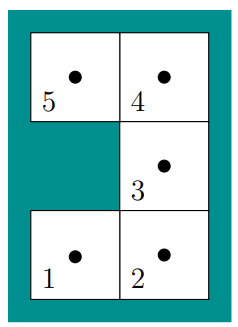
\includegraphics[width=3cm]{Localization_Example.png}
    \caption{This example shows the possible moves of a robot to which grids he could move. \cite{planning_algorithms_steven_m_lavalle}}
    \label{fig:Localization Example}
\end{figure}

With different sensors like a compass and a camera, it is possible to define a position. Further information on localization can be read in the mentioned book. The environment uncertainty and mapping topic focus on how to define an environment when there is no map given so that the robot has to act upon sensors only. \cite{planning_algorithms_steven_m_lavalle}

\subsection{Planning under Differential Constraints} \label{sec:Planning under Differential Constraints}
This section covers differential constraints—local limitations like allowable velocities at each point. Differential constraints are mostly from kinematics and dynamics. Smoothness is a weak differential constraint, while obstacles are global constraints.

\textbf{Differential Models} covers examples of velocity constraints in state space. There are two ways of differential constraints: parametric and implicit. Implicit expresses prohibited velocities and are more general, whereas parametric representation expresses allowed velocities. A simple car has three degrees of freedom, as shown in figure \ref{fig:Simple Car Velocity Space}.
\begin{figure}[H]
    \centering
    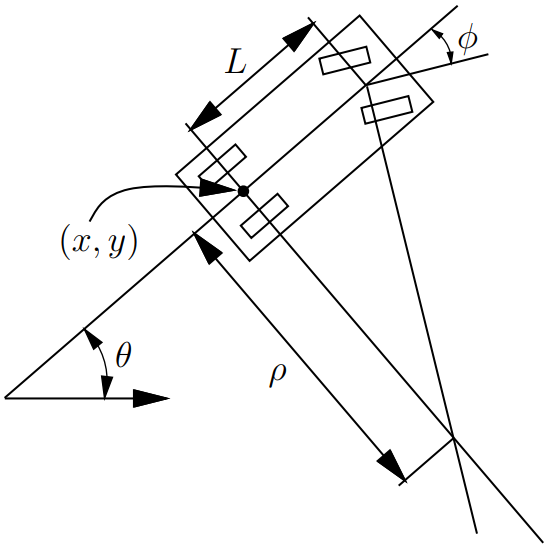
\includegraphics[width=6cm]{Simple_Car_Velocity_Space.png}
    \caption{This example shows possible moves of a robot to which grids he could move to. \cite{planning_algorithms_steven_m_lavalle}}
    \label{fig:Simple Car Velocity Space}
\end{figure}
The velocity is two-dimensional, on the other hand. Therefore, the dimensions must be shrunken down from three to two. There are also concepts of multiple decision-makers, which are not covered in this thesis.

\textbf{Sampling-Based Planning Under Differential Constraints} covers the satisfaction of differential constraints with an initial and goal state. Constraints like continuity or smoothness can be applied as well. Kinodynamic planning is a motion planning problem with velocity and acceleration bounds. On the other hand, trajectory planning deals with a velocity and path function. There can also be collision constraints with obstacles, for example.
Reachable sets describe what has to be visited, there could also be time-limited reachable sets. A reachability graph can help to visualize which sets are already visited like the one in figure \ref{fig:Reachability Graph}.
\begin{figure}[H]
    \centering
    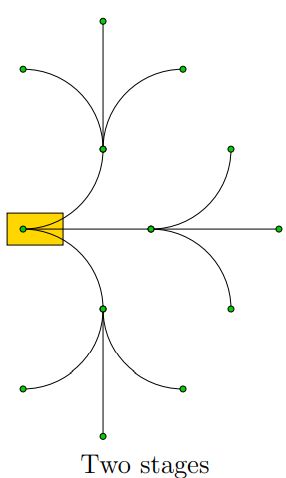
\includegraphics[width=4cm]{Reachability_Graph.png}
    \caption{This figure shows how a reachability graph can be visualized and represents two stages. \cite{planning_algorithms_steven_m_lavalle}}
    \label{fig:Reachability Graph}
\end{figure}
Local planning by having smaller problems that can be solved locally to solve the bigger problem. The following pseudocode snipped in listing \ref{lst:Simple RDT with differential constraints} shows how the \acrlong{rdt} (\acrshort{rdt}) can be used for calculating a path under differential constraints.
\begin{lstlisting}[mathescape=true, caption={The local planning method computes $x_r$. A new vertex will be available: $x_r$. \cite{planning_algorithms_steven_m_lavalle}}, label={lst:Simple RDT with differential constraints}]
SIMPLE RDT WITH DIFFERENTIAL CONSTRAINTS($x_0$)
 1 G.init($x_0$);
 2 for i = 1 to k do
 3 $x_n$ $\leftarrow$ nearest($S(G), \alpha(i)$);
 4 ($\widetilde{u}^p$, $x_r$) $\leftarrow$ local planner($x_n$, $\alpha(i)$);
 5 G.add vertex($x_r$);
 6 G.add edge($\widetilde{u}^p$);
\end{lstlisting}
Randomized potential fields can also be a method for sampling-based planning under differential constraints, which is not covered in this thesis. Path constraints can also narrow down the trajectory, like the turning angle. \cite{planning_algorithms_steven_m_lavalle}

\textbf{System Theory and Analytical Techniques} takes the physics of the robot into account. Since this thesis covers trajectory or path planning, this section would be out of scope. \cite{planning_algorithms_steven_m_lavalle}
